\documentclass[twocolumn]{svjour3}

\setcounter{tocdepth}{3}
\usepackage{algorithm}
\usepackage{algpseudocode}
\usepackage[fleqn]{amsmath} % flush equations left
\usepackage{amssymb}
\usepackage{array,url}
\usepackage{authblk}
\usepackage{caption}
\usepackage{courier}
\usepackage{enumitem}
\usepackage{graphicx}
\usepackage{helvet}
\usepackage{multicol}
\usepackage{multirow}
%\usepackage{sectsty}
\usepackage{subcaption}\captionsetup{compatibility=false}
\usepackage{tabularx}
\usepackage{tikz}\usetikzlibrary{arrows, backgrounds}
\usepackage{times}
\usepackage{url}
\usepackage{xcolor}
\usepackage{fancyvrb}
\usepackage{changepage}
\usepackage{algorithm}% http://ctan.org/pkg/algorithms
\usepackage{algpseudocode}% http://ctan.org/pkg/algorithmicx
\newcommand{\var}[1]{{\ttfamily#1}}% variable

% change the appearance of the tikz arrow for the argumentation networks
% and some other settings to make all the graphs look similar
\tikzset{>=latex,every node/.style={circle, minimum size=0.5cm, draw=black}}

% Tikz stuff for arguments with GRL
\tikzset{
  argNodeIN/.style={shape=rectangle,draw,fill=white,align=center},
  argNodeOUT/.style={shape=rectangle, draw=black!60, text=black!40,fill=white},
  traceNodeRED/.style={circle,draw=black, fill=red, inner sep=0pt,minimum size=8pt},
  traceNodeGREEN/.style={circle,draw=black, fill=green, inner sep=0pt,minimum size=8pt},
  attackLink/.style={draw=black,->,line width=0.5mm},
  traceLinkRED/.style={draw, densely dotted,-,line width=0.5mm, draw=red},
  traceLinkGREEN/.style={draw, densely dotted,-,line width=0.5mm, draw=green},
  CQLink/.style={line width=0.5mm, dotted,->},
  ldots/.style={draw=none,rotate=90,font=\fontsize{20}{22.4}\selectfont},
  grl/.style={draw=none},
  disabled/.style={opacity=0.5}
}
\newcommand{\argtext}[2]{
\begin{tabularx}{0.2\textwidth}{X}
\ifx&#1&%
\else
\textbf{(#1)}
\fi
#2
\end{tabularx}
}
\newcommand{\smallargtext}[2]{
\begin{tabularx}{0.25\textwidth}{X}
\ifx&#1&%
\else
\textbf{(#1)}
\fi
#2
\end{tabularx}
}
\newcommand{\longargtext}[2]{
\begin{tabularx}{0.5\textwidth}{X}
\ifx&#1&%
\else
\textbf{(#1)}
\fi
#2
\end{tabularx}
}

% rationale
\newcommand{\rationale}{\emph{Rationale and example:}}


%\addtolength{\oddsidemargin}{-0.85in}
%\addtolength{\evensidemargin}{-0.85in}
%\addtolength{\textwidth}{1.7in}
%\addtolength{\topmargin}{-.7in}
%\addtolength{\textheight}{1.3in}
%\setlength{\columnsep}{0.3in}
\newcommand{\Mark}[1]{\textsuperscript{#1}}

% TODO command
\newcommand\todo[4][]{%
	\ifthenelse{\equal{#1}{resolved}}{%
		% nothing
	}{%
		{\bf\color{red}TODO for #3\textcolor{gray}{(by #2)}: #4}%
	}%
}

\algnewcommand\algorithmicswitch{\textbf{switch}}
\algnewcommand\algorithmiccase{\textbf{case}}
\algnewcommand\algorithmicassert{\texttt{assert}}
\algnewcommand\Assert[1]{\State \algorithmicassert(#1)}%
% New "environments"
\algdef{SE}[SWITCH]{Switch}{EndSwitch}[1]{\algorithmicswitch\ #1\ \algorithmicdo}{\algorithmicend\ \algorithmicswitch}%
\algdef{SE}[CASE]{Case}{EndCase}[1]{\algorithmiccase\ #1}{\algorithmicend\ \algorithmiccase}%
\algtext*{EndSwitch}%
\algtext*{EndCase}%


% TO TURN OFF TODOS UNCOMMENT THE FOLLOWING:
% \renewcommand\todo[4][]{}

% use like this:
% \todo{floris}{marc}{Can you please update figure 2?} - Floris is asking Marc to update figure 2, this will show in red in the PDF
% \todo[resolved]{floris}{marc}{done} - Marc has updated fig 2 (or gives a reason why he doesn't want to uppdate the figure. This will show only in the tex


\renewcommand\Authfont{\fontsize{10}{14.4}\selectfont}
\renewcommand\Affilfont{\fontsize{9}{10.8}\selectfont}

%\sectionfont{\fontsize{12}{15}\selectfont}
%\subsectionfont{\fontsize{10}{15}\selectfont}

\begin{document}\sloppy
\twocolumn[{%
 \centering
 \LARGE RationalGRL: A Framework for Argumentation and Goal Modeling \\[1.5em]
 \large Marc van Zee\Mark{1},
        Floris Bex\Mark{2}
        and Sepideh Ghanavati\Mark{3}\\[1em]
 \normalsize
 \begin{tabular}{*{3}{>{\centering}p{.33\textwidth}}}
  \Mark{1}Computer Science and Communication (CSC) & \Mark{2}Department of Information and Computing Sciences & \Mark{3}Department of Computer Science  \tabularnewline
  University of Luxembourg & Utrecht University & Texas Tech University \tabularnewline
  \url{marcvanzee@gmail.com} & \url{f.j.bex@uu.nl} & \url{sepideh.ghanavati@ttu.edu}
 \end{tabular}\\[3em] % some more space after the title part
}]

\begin{abstract}
Goal modeling languages capture the relations between an information system and its environment using high-level goals and their relationships with lower level goals and tasks. The process of constructing a goal model usually involves discussions between a requirements engineer and a group of stakeholders. While it is possible to capture part of this discussion process in the goal model, for instance by specifying alternative solutions for a goal, not all of the arguments can be found back in the resulting model. For instance, reasons for accepting or rejecting an element or a relation between two elements are not captured. In this paper, we investigate to what extent argumentation techniques from artificial intelligence can be applied to goal modeling. We apply the argument scheme for practical reasoning (PRAS), which is used in AI to reason about goals to the Goal-oriented Requirements Language (GRL). We develop a formal metamodel for the new language, link it to the GRL metamodel, and we implement our extension into jUCMNav, the Eclipse-based open source tool for GRL.
\end{abstract}
%SG: what are the findings? or what case study we are using?

\newpage

\paragraph{Keywords} Goal modeling $\cdot$ Argumentation $\cdot$ Practical Reasoning $\cdot$ Goal-oriented requirements engineering

\section{Introduction}
\label{sect:introduction}

\subsection{Requirements Engineering and Goal Modeling}

Requirements Engineering (RE) is an approach to assess the role of a future information system within a human or automated environment. An important goal in RE is to produce a consistent and comprehensive set of requirements covering different aspects of the system, such as general functional requirements, operational environment constraints, and so-called non-functional requirements such as security and performance. 

One of the first activities in RE are the ``early-phase'' requirements engineering activities, which include those that consider how the intended system should meet organizational goals, why it is needed, what alternatives may exist, what implications of the alternatives are for different stakeholders, and how the interests and concerns of stakeholders might be addressed~\cite{yu1997towards}. These activities fall under the umbrella of goal modeling. The are a large number of established RE methods using goal models in the early stage of requirements analysis (e.g.,~\cite{liu2004designing,donzelli2004goal,dardenne1993goal,chung2012non,castro2002towards}, overviews can be found in~\cite{van2001goal,kavakliL05}). Several goal modeling languages have been developed in the last two decades as well. The most popular ones include $i*$~\cite{Yu:1997:TMR:827255.827807}, Keep All Objects Satisfied (KAOS)~\cite{van2008requirements}, the NFR framework~\cite{chung2012non}, \textsc{Tropos}~\cite{giorgini2005goal}, the Business Intelligence Model (BIM)~\cite{horkoff2014strategic}, and the Goal-oriented Requirements Language (GRL)~\cite{Amyot:2010:EGM:1841349.1841356}.

\subsection{Problem Statement}
\label{sect:problem_statement}


A goal model is often the result of a discussion process between a group of stakeholders. For small-sized systems, goal models are usually constructed in a short amount of time, involving stakeholders with a similar background. Therefore, it is often not necessary to record all of the details of the discussion process that led to the final goal model. However, most real-world information systems -- e.g., air-traffic management, industrial production processes, or government and healthcare services -- are complex and are not constructed in a short amount of time, but rather over the course of several workshops. In such situations, failing to record the discussions underlying a goal model in a structured manner may harm the success of the RE phase of system development for various reasons stated below. 

First, it is well-known that stakeholders' preferences are rarely absolute, relevant, stable, or consistent~\cite{march1978bounded}. Therefore, it is possible that a stakeholder changes his or her opinion about a modeling decision in between two goal modeling sessions, which may require revisions of the goal model. If previous preferences and opinions are not stored explicitly, it is not possible to remind stakeholders of their previous opinions which results in having unnecessary discussions and revisions. As the number of participants increases, revising the goal model based on changing preferences can take up a significant amount of time. 

Second, other stakeholders, such as new developers on the team who were not the original authors of the goal model, may have to make sense of the goal model, for instance, to use it as an input in a later RE stage or at the design and development phase. If these users have no knowledge of the underlying rationale of the goal model, it may not only be more difficult to understand the model, but they may also end up having the same discussions as the previous group of stakeholders.

Third, alternative and different ideas and opposing views that could potentially have led to different goal diagrams could be lost. For instance, a group of stakeholders specifying a goal model for a user interface may decide to reduce softgoals ``easy to use'' and ``fast'' to one softgoal ``easy to use''. Thus, the resulting goal model merely contains the softgoal ``easy to use'', but the discussion as well as the decision to reject ``fast'' are lost. This leads to a poor understanding of the problem and solution domain. In fact, empirical data suggest that this is an important reason of RE project failure~\cite{curtis1988field}. 

Fourth and lastly, in goal models in general, ``rationale'' behind any decision is static and does not immediately impact the goal models when they change. That is, current goal modeling languages have limited support for reasoning about changing beliefs and opinions, and their effect on the goal model. A stakeholder may change his or her opinion, but it is not always directly clear what its effect is on the goal model. Similarly, a part of the goal model may change, but it is not possible to formally reason about the consistency of this new goal model with the underlying beliefs and arguments in the goal modeling languages. This becomes more problematic if the participants constructing the goal model change, since modeling decisions made by one group of stakeholders may conflict with the underlying beliefs put forward by another group of stakeholders.

\subsection{Research Questions}
 
The aim of this research is to resolve the above issues by developing a framework with a tool-support, which combines goal modeling approaches with argumentation techniques from Artificial Intelligence (AI) research\cite{atkinson2007}. We have identified five important requirements for our framework: 
\begin{enumerate}
\item The argumentation techniques should be close to the actual discussions of stakeholders or designers in the early requirements engineering phase.
\item 
The framework must have formal traceability links between elements of the goal model and underlying arguments.
\item 
Using these traceability links, it must be possible to compute the effect of changes in the goal model on the underlying arguments, and vice versa.
\item 
The framework must have a tool support.
\item 
There should be a methodology for the framework to guide the practitioners in its application in real cases.
\end{enumerate}

The five requirements above serve as the success criteria of our approach. That is, if our framework satisfies these requirements, we reach our goal. 

In this context, the main research question is: 

\begin{quote}
\textbf{RQ.} What are the constructs, mechanisms and rules for developing a framework that formally captures the discussions between stakeholders such that it can generate goal models?
\end{quote}

%The five requirements above are the success criteria of our approach, that is, the satisfaction of the six requirements will result in a positive answer to the research question.

\todo{Sepideh}{Marc}{Read this paragraph and see if it makes sense.}
To answer the research question above and solve some of the concerns mentioned in Subsection~\ref{sect:problem_statement}, we propose a framework called RationalGRL. The RationalGRL framework combines the Goal-oriented Requirements Language (GRL) with a technique from argumentation and discourse modeling called \emph{argument schemes}~\cite{walton-etal2004}. 

In past, we introduced our preliminary steps towards RationalGRL framework~\cite{bnaic2014,vanzee-etal:renext2015,vanZee-etal:er2016} with its tool-support~\cite{vanZee-etal:comma2016}.  In our previous work, argument diagrams are integrated with GRL models to allow better representation of stakeholder's arguments and discussions. In our current paper, we improve RationalGRL framework by adding argument schemes and critical questions to argumentation framework and provide traceability links between the argumentation framework and GRL.  For this, we modify and extend our metamodel to specify how our framework extends GRL, and we use this as the basis for a prototype web-based implementation~\footnote{The tool is available at <GITHUB LINK>}. %SG: Placeholder for the link. 
We develop an initial list of argument schemes and critical questions by analyzing a set of transcripts containing discussion about an information system. Our framework is fully extensible, meaning that argument schemes and critical questions can be added by users for specific problem domains. We develop a methodology for using RationalGRL, which consists developing goal models and posing arguments in an integrated way. This methodology is intended to be used by practitioners in the field. We formalize RationalGRL using propositional logic, and develop algorithms for adding goal elements and arguments. We illustrates the steps of our framework  and how the framework can be applied in real cases with a traffic simulator example.

\subsection{Organization} %SG: Will get back to this at the end of the paper.

This article is organized as follows. Section~\ref{sect:background} contains background and introduces our running example, the Goal-oriented Requirements Language (GRL)~\cite{Amyot:2010:EGM:1841349.1841356}, and argument schemes. Section~\ref{sect:overview} provides a brief and high-level overview of our framework, together with a metamodel and the methodology. Section~\ref{sect:gmas} contains an in depth explanation of how we obtained an initial set of argument schemes by annotating transcripts from discussions about an information system, and in Section~\ref{sect:examples} we provide several examples of these arguments schemes. In Section~\ref{sect:formalframework} we formalize RationalGRL and our arguments schemes using propositional logic and we use well-known argumentation semantics to compute which arguments are accepted and which are rejected. We also develop various algorithms for the argument schemes in this section. In Section~\ref{sect:tool} we provide a brief overview of the prototype tool we developed for RationalGRL. Finally, Section~\ref{sect:discussion} contains a discussion, covering related work, future work, and a conclusion.
\section{Background: Goal-oriented Requirements Language and argument schemes}
\label{sect:background}

In this section, we first introduce our running example, after which we introduce the Goal-oriented Requirements Language (GRL)~\cite{Amyot:2010:EGM:1841349.1841356}, which is the goal modeling language we use to integrate with the argumentation framework. Next, we introduce argument schemes, and in particular, we discuss the \emph{practical reasoning argument scheme (PRAS)}~\cite{atkinson2007}, which is an argument scheme that is used to form arguments and counter-arguments about situations involving goals. Finally, we give an overview of the integration between PRAS and GRL.  %This will be our starting point in the next section.

\subsection{Running example: Traffic Simulator}
\label{sect:goals:runningexample}

We use the traffic simulator design case to explain the concepts and the framework in this paper. Traffic simulator design is the topic of discussion in the transcripts used for argumentation framework.   
%Most of the examples in this article, as well as the topic of discussion in the transcripts we analyze, come from the traffic simulator design exercise. 
In this exercise, designers are provided with a problem description, requirements, and a description of the desired outcomes. The problem description is given in full in Appendix~\ref{sect:designprompt}, and is summarized as follows: The client of the project is Professor E, who teaches civil engineering courses at an American university. In order for the professor to teach students how various theories (such as queuing theory) around traffic lights work, a software analyst is hired to specify the goal and requirements of the system. %and It is the task of the designer to specify a system in which the professor can teach students how various theories around traffic lights works, such as queuing theory. 
To this end, a piece of software will be developed in which students can create visual maps of an area, regulate traffic, and so forth. The original version of the problem descrption~\cite{UCIworkshop} is well known in the field of design reasoning and it has been used in a workshop\footnote{\url{http://www.ics.uci.edu/design-workshop/}}. Transcripts of this workshop have been analyzed in detail~\cite{Petre:2013:SDA:2535028}. Although the concepts of traffic lights, lanes, and intersections are common and appear to be simple, building a traffic simulator to represent these relationships and events in real time turns out to be challenging.

\subsection{Goal-oriented Requirements Language (GRL)}
\label{sect:background:grl}
GRL is a visual modeling language for specifying intentions, business goals, and \emph{non-functional requirements} of multiple stakeholders \cite{Amyot:2010:EGM:1841349.1841356}. GRL is part of the User Requirements Notation, an ITU-T standard, that combines goals and non-functional requirements with functional and operational requirements (i.e. use case maps) in one. GRL can be used to specify alternatives that have to be considered, decisions that have been made, and rationales for making decisions. A GRL model is a connected graph of intentional elements that optionally are part of the actors. All the elements and relationships used in GRL are shown in Figure~\ref{fig:grl_legend}.

\begin{figure}[ht]
\centering
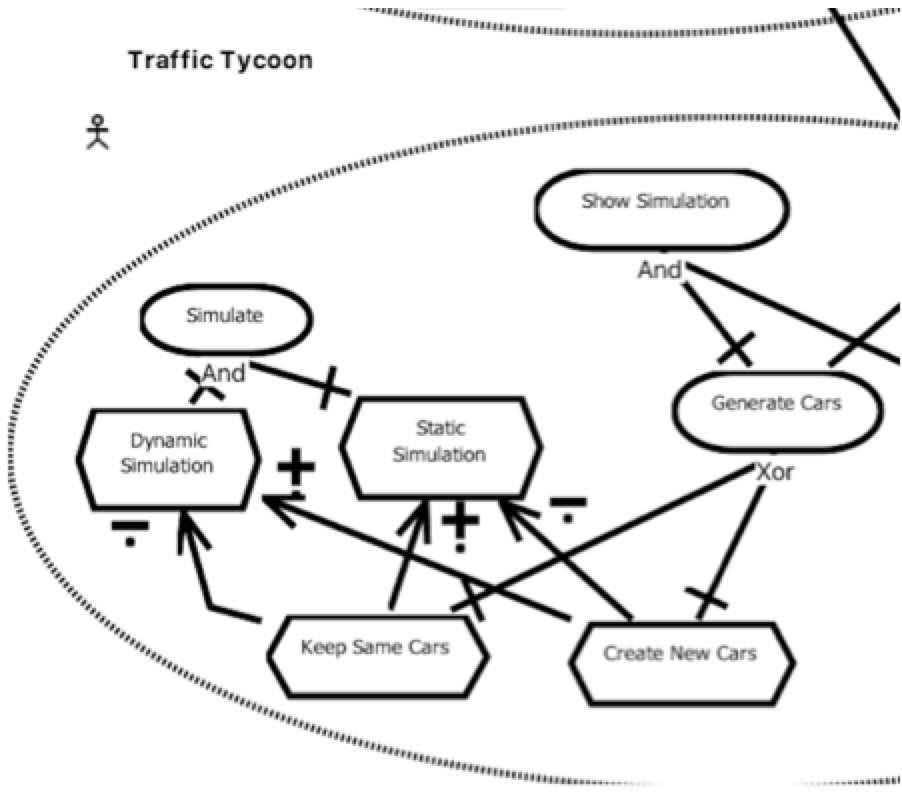
\includegraphics[width=0.5\textwidth]{img/example_small}
\caption{Partial GRL Model of Traffic Simulator Example %(\todo{Marc}{Sepideh}{Turn into vector image, turn ``Dynamic simulation'' and ``Static Simulation'' into goals, turn ``Simulate'' into softgoal, add some resource}}
\label{fig:example-small}
\end{figure} %SG: I changed the figure a bit so that we won't need to change Figure 10. Let me know if you still want to change them according to the above.

\begin{figure*}[ht]
\centering
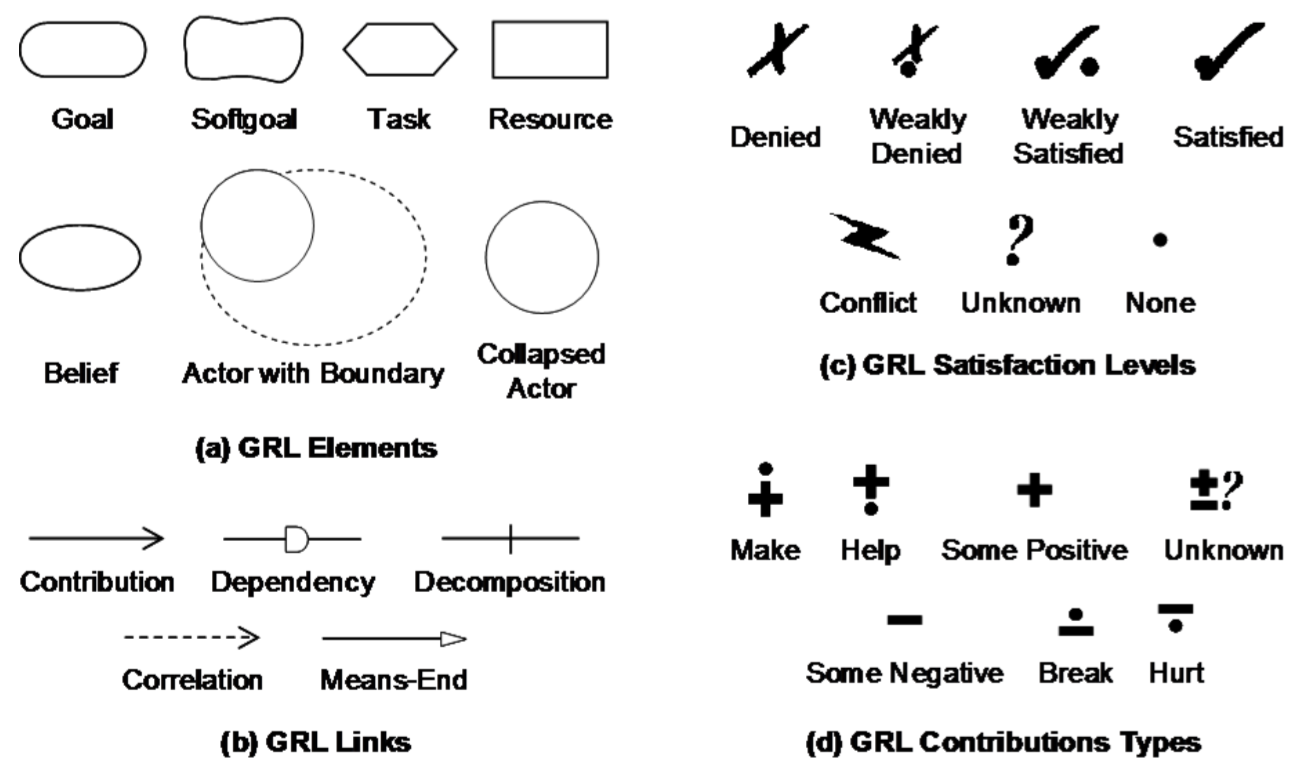
\includegraphics[scale=0.6]{img/grl_legend}
\caption{Basic elements and relationships of GRL}
\label{fig:grl_legend}
\end{figure*}

Figure~\ref{fig:example-small} illustrates a partial GRL diagram from the traffic simulator design exercise (the full figure is shown in Figure~\ref{fig:transcripts:grl} and will be discussed in Section~\ref{sect:gmas}). An actor (
\includegraphics[scale=1]{img/actor}) represents a stakeholder of a system or the system itself (\texttt{Traffic Tycoon}, Figure~\ref{fig:example-small}). Actors are holders of intentions; they are the active entities in the system or its environment who want goals to be achieved, tasks to be performed, resources to be available, and softgoals to be satisfied. Softgoals (
\includegraphics[scale=1]{img/softgoal}) differentiate themselves from goals (
\includegraphics[scale=1]{img/goal}) in that there is no clear, objective measure of satisfaction for a softgoal whereas a goal is quantifiable, often in a binary way. Softgoals (e.g. \texttt{Show Simulation}) are often related to non-functional requirements, whereas goals (such as  \texttt{Generate cars}) are related to functional requirements. Tasks (
\includegraphics[scale=1]{img/task}) represent solutions to (or operationalizations of) goals and softgoals. In Figure~\ref{fig:example-small}, some of the tasks are  \texttt{Create new cars} and \texttt{Keep same cars}. In order to be achieved or completed, softgoals, goals, and tasks may require resources (
\includegraphics[scale=1]{img/resource}) to be available (e.g., \texttt{External Library}).

Different links connect the elements in a GRL model. AND, IOR (Inclusive OR), and XOR (eXclusive OR) decomposition links (
\includegraphics[scale=1]{img/decomposition}) allow an element to be decomposed into sub-elements. In Figure~\ref{fig:example-small}, the goal \texttt{Generate cars} is XOR-decomposed to the tasks \texttt{Create new cars} and \texttt{Keep same cars}. Contribution links (
\includegraphics[scale=1]{img/contribution}) indicate desired impacts of one element on another element. A contribution link has a qualitative contribution type or a quantitative contribution. Task  \texttt{Create new cars} has a \emph{help} qualitative contribution to the task \texttt{Dynamic Simulation}. Dependency links (
\includegraphics[scale=1]{img/dependency}) model relationships between actors. The goal \texttt{Generate Cars} depends on the goal \texttt{Value Has Changed}. %SG: I added it to the model but we can also remove it altogether. 
%\todo{Marc}{Sepideh}{Shall we add a dependency relation as well? They don't play a big role in our work..}

GRL is based on $i*$~\cite{Yu:1997:TMR:827255.827807} and the NFR Framework~\cite{chung2012non}, but it is not as restrictive as $i*$. Intentional elements and links can be more freely combined, the notion of agents is replaced with the more general notion of actors, i.e., stakeholders, and a task does not necessarily have to be an activity performed by an actor, but may also describe properties of a solution. GRL has a well-defined syntax and semantics. Furthermore, GRL provides support for providing a scalable and consistent representation of multiple views/diagrams of the same goal model (see~\cite[Ch.2]{Ghanavati2013} for more details). GRL is also linked to Use Case Maps via URNLink ((
\includegraphics[scale=1]{img/urnlink}) which provides traceability between concepts and instances of the goal model and behavioral design models. Multiple views and traceability links are a good fit with our current research: we aim to add traceability links between intentional elements and their underlying arguments. 

GRL has six evaluation algorithms which are semi-automated and allow the analysis of alternatives and design decisions by calculating the satisfaction value of the intentional elements across multiple diagrams quantitatively, qualitatively or in a hybrid way. The satisfaction values from intentional elements in GRL can also be propagated to the elements of Use Case Maps.  jUCMNav, GRL tool-support, also allows for adding new GRL evaluation algorithms~\cite{jUCMNav}. GRL also has the capability to be extended through metadata, links, and external OCL constraints. This allows GRL to be used in many domains without the need to change the whole modeling language. This feature also helps us apply our argumentation to other domains such as compliance, which we explain in more detail in Section~\ref{sect:goalmodeling:openissues}.

The GRL model in Figure~\ref{fig:example-small} shows the softgoals, goals, tasks and the relationship between the different intentional elements in the model. However, the rationales and arguments behind certain intentional elements are not shown in the GRL model. Some of the questions that might be interesting to know about are the following:

\begin{itemize}
	\item Why does actor \texttt{Traffic Tycoon} have only a single softgoal \texttt{Show Simulation}? Why is this, for instance, not connected to goal \texttt{Simulate}? %SG: I changed this question but let me know if you want to change them back and then change the graph.
	\item What does \texttt{Keep same cars} mean?
	\item Why does task \texttt{Keep same cars} contribute positively to \texttt{Static simulation} and negatively to \texttt{Dynamic simulation}?
	\item Why does \texttt{Generate Cars} XOR-decompose into two tasks?
\end{itemize}

These are the type of the questions that we cannot answer by just looking at GRL models. The model in Figure~\ref{fig:example-small} does not contain information about discussions that lead to the resulting model, such as various clarification steps for the naming, or alternatives that have been considered for the relationships. In this article we aim to address this shortcoming.

\subsection{Argument Scheme for Practical Reasoning (PRAS)}
\label{sect:background:pras}

Reasoning about which goals to pursue and actions to take is often referred to as \emph{practical reasoning}, and has been studied extensively in philosophy (e.g. \cite{Raz1978-RAZPR,walton1990}) and artificial intelligence \cite{bratman1987,atkinson2007}. One approach is to capture practical reasoning using arguments schemes and critical questions~\cite{walton1990}. Applying an argument schemes results in an argument in favor of, for example, taking an action. This argument can, then, be tested with critical questions about, for instance, whether the action is possible given the situation. A negative answer to such a question leads to a counterargument to the original argument for the action. 

Atkinson et al.~\cite{atkinson2007} develop an argument scheme for practical reasoning, which they call the \emph{Practical Reasoning Argument Scheme} (PRAS). This argument scheme is as follows\footnote{The original argument schemes uses slightly different terminology: we have replaced \emph{value} with \emph{softgoal}. Our results do not depend on these adjustments, but they make the relation between PRAS and GRL more clear.}:

\begin{itemize}
\item[] We have goal $G$,
\item[] Doing action $A$ realizes to goal $G$,
\item[] Which will contribute positively to the softgoal $S$
\item[] \textit{Therefore} 
\item[] We should perform action $A$
\end{itemize}

The capital letters $G$, $A$, and $S$ are variables, which can be instantiated with concrete goals, actions, and softgoals. Once instantiated, we obtain an argument. We can for instance instantiate the argument scheme above with the elements of Figure~\ref{fig:example-small} as follows: %SG: Need to update the example.
\begin{itemize}
\item[] We have goal \texttt{Static simulation},
\item[] Doing action \texttt{Keep same cars} realizes goal \texttt{Static simulation}, 
\item[] Which contribute positively to the softgoal \texttt{Simulate} 
\item[] \textit{Therefore} 
\item[] We should perform action \texttt{Keep same cars}.
\end{itemize}

Atkinson \emph{et al.}~\cite{atkinson2007} define a set of critical questions that point to typical ways in which a practical argument can be criticized by, for example, questioning the validity of the elements in the scheme or the connections between the elements. Some examples of critical questions are as follows.

\begin{enumerate}
\item Will the action realize the desired goal?
\item Are there alternative ways of realizing the same goal?
\item Are there alternative ways of contributing to the same softgoal?
\item Does performing the action contribute negatively to some other softgoal?
\item Is the action possible?
\item Can the desired goal be realized?
\item Is the softgoal indeed a legitimate softgoal?
\end{enumerate}

These critical questions can point to new arguments that might counter the original argument. Take, for example, critical question 1: if we find that  \texttt{Keep same cars} actually does not realize goal \texttt{Static Simulation}, we can form a counter-argument. %SG:placeholder for the examples. 

Another way to elaborate an argument for an action is to suggest an alternative action that realizes the same goal (question 2) or an alternative goal that contributes to the same softgoal (question 3). For example,  can argue that another goal \texttt{Semi-dynamic Simulation} also realizes the softgoal \texttt{Simulate}.
\todo{Marc}{Sepideh}{Do you think our example is good? I think it is confusing. Perhaps we should just create an artificial example here, loosely based on the traffic simulator but where the model makes sense to the reader. Now the tasks are all a bit vague and I think nobody knows what they actually mean.}

In argumentation, counterarguments are said to \emph{attack} the original arguments (and sometimes vice versa). In the work of Atkinson et al.~\cite{atkinson2007}, arguments and their attacks are captured as an \emph{argumentation framework} of arguments and attack relations as introduced by Dung~\cite{Dung1995}. Given an argumentation framework, once can compute very precisely which arguments are accepted and which are rejected. 

\subsection{Combining PRAS and GRL}
\label{sect:background:pras:motivation}

The usefulness of argument schemes, and PRAS in particular, for the analysis of practical reasoning situations has been shown in different areas such as e-democracy~\cite{cartwright2009IS}, law~\cite{atkinson2005legal}, planning \cite{medellin2013planning} and choosing between safety critical actions \cite{tolchinsky2012deliberation}. In this article, we aim at capturing the stakeholder's discussions as formal argumentation based on PRAS to decide whether intentional elements and their relationships are shown in the resulting goal model. This approach provides a rationalization to the elements of the goal model in terms of underlying arguments, and furthermore, it helps understanding why certain other elements have been rejected.

Argumentation schemes and their associated critical questions are very well suited for modeling discussions about a goal model: as Murukannaiah et al.~\cite{murukannaiah2015} have shown, they can guide users in systematically deriving conclusions and making assumptions explicit. This can also be seen from the obvious similarities between PRAS (actions, goals, values) and GRL (tasks, goals, softgoals) in the example above.

However, there are also some differences between PRAS and GRL. Not all elements and relationships of GRL fit into PRAS. For instance, PRAS does not have a notion of ``resource'', and many of the relationships of GRL do not occur in PRAS. Furthermore, it is not directly clear whether the critical questions as proposed by Atkinson can actually apply to GRL. Therefore, we develop our own set of argument schemes and critical questions in Section~\ref{sect:gmas} by analyzing transcripts of discussions about the traffic simulator. Before doing so, we give an overview of our framework in the next section.
\section{Argument Schemes for Goal Modeling: a Case Study}
\label{sect:gmas}

Recall that \textbf{requirement 1} of our RationalGRL framework is that the argumentation techniques should be close to the actual discussions of stakeholders or designers in the early requirements engineering phase. To get a sense of such discussions, we performed an extensive case study to see which types of discourse are used during a discussion of system requirements, and how these discourse types can be captured as argument schemes and critical questions regarding goals and tasks. We manually coded transcripts of such discussions using a list of argument schemes and critical questions based on GRL and PRAS. In this section we present our case study. All original transcripts, codings, and models are available in our online repository, which can be found at:  
 
\begin{quote}
\url{Marc please insert URL}
\end{quote}

In order to obtain actual requirements discussions, we turned to a recent series of experiments by Schriek et al. \cite{SchriekEtal2016}. In these experiments, 12 groups of two or three students in a Software Architecture course at MSc level were given the traffic simulator assignment (Appendix~\ref{sect:designprompt}). These groups had a maximum of two hours to design a traffic simulator, which included a discussion of the requirements of this traffic simulator. The students did not use any goal modeling technique in the course or during the discussions. The students were asked to record their design sessions, and the recordings were subsequently transcribed. We used three of these transcripts, totaling 153 pages, for our case study. 


\begin{table}[t]
\centering
\begin{tabularx}{0.5\textwidth}{|l|X|l|l|l|>{\bfseries}l|}
\hline
\multicolumn{2}{|c|}{\textbf{Scheme/Question}} & $t_1$ & $t_2$ & $t_3$ & \textbf{total}\\
\hline 
AS0 & Actor & 2 & 2 & 5 & 9\\
\hline
AS1 & Resource & 2 & 4 & 5 & 11\\
\hline
AS2 & Task/action & 20 & 21 & 17 & 58\\
\hline
AS3 & Goal & 0 & 2 & 2 & 4\\
\hline
AS4 & Softgoal & 3 & 4 & 2 & 9\\
\hline
AS5 & Goal decomposes into tasks & 4 &0& 4 & 8\\
\hline
AS6 & Task contributes (negatively) to softgoal & 8 & 3 &0& 11\\
\hline
AS7 & Goal contributes (negatively) to softgoal &0& 1 & 1 & 2\\
\hline
AS8 & Resource contributes to task & 0 & 4 & 3 & 7\\
\hline
AS9 & Actor depends on actor &0& 1 & 3 & 4\\
\hline
AS10 & Task decomposes into tasks & 11 &14 &11 &36\\ 
\hline
\hline
CQ2 & Task is possible? & 2 & 2 & 1 & 5\\
\hline		
CQ5a & Does the goal decompose into the tasks? & 0 & 1 & 0 & 1\\
\hline
CQ5b & Goal decomposes into other tasks? & 1 & 0 & 0 & 1\\
\hline
CQ6b & Task has negative side effects? & 2 & 0 & 0 & 2\\
\hline
CQ10a & Task decompose into other tasks? & 1 &2 &0&3\\
\hline
CQ10b & Decomposition type correct? &1 &0& 1 &2\\
\hline
\hline
CQ11 & Is the element relevant/useful? & 2 & 3 & 2 &7\\
\hline
CQ12 & Is the element clear/unambiguous? &3 &10 & 3 & 16\\
\hline
\hline
- & Generic counterargument & 0& 2 & 2 & 4\\
\hline
\hline
\multicolumn{2}{|c|}{\textbf{TOTAL}}&69&80&69&222\\
\hline
\end{tabularx}
\caption{Occurrences of argument schemes and critical questions in the transcripts.}
\label{table:transcripts:results:argumentschemes}
\end{table}

Before we started coding the transcripts, we drew up an initial list of 10 argument schemes (AS0-AS9 in Table~\ref{table:transcripts:results:argumentschemes}), representing \emph{claims} about the goal model containing the requirements of the system. AS0 to AS4 are schemes that concern a single element of the goal model. So, for example, AS0 represents the claim `$a$ is a relevant actor for the system', and AS3 represents the claim `$G$ is a goal for the system'. AS5 to AS9 are claims about the links between GRL elements. Our initial list also contained 18 critical questions, inspired by the questions associated with the original Practical Reasoning Argumentation Scheme \cite{atkinson2007}. CQ2 to CQ6b (Table~\ref{table:transcripts:results:argumentschemes}) are examples of these critical questions, other examples are `Is the softgoal legitimate?' and `Are there alternative ways to contribute to the same softgoal?'.

%%TODO check numbers against original annotation docs
Using the initial list of arguments and critical questions, we coded three transcripts of requirements discussions. The codings were performed by one author and subsequently checked by another author. As the transcripts contain spoken language, the codings involved some interpretation. For example, the students almost never literally say `actor $a$ has task $T$'. Rather, they say things such as `...we have a set of actions. Save map, open map, ...' (Table~\ref{table:transcripts:traffic-light}, Appendix~\ref{sect:transcripts:excerpts}) and `... in that process there are activities like create a visual map, create a road' (Table~\ref{table:transcript:task-clarification}, Appendix~\ref{sect:transcripts:excerpts}). Furthermore, in some cases the critical questions are explicit. For example, CQ10b is found in the transcripts as `...is this an OR or an AND?' (Table \ref{table:transcript:decomposition}, Appendix~\ref{sect:transcripts:excerpts}). In other cases, however, the question remains implicit but we added it in the coding. For example, CQ12 is not found in the transcripts, but the related counterargument is:  `...you don't have to specifically add a traffic light' (Table~\ref{table:transcripts:traffic-light}, Appendix~\ref{sect:transcripts:excerpts}). 

During the coding, new argument schemes and critical questions were added to the list. For example, we found that the discussants often talk about tasks decomposing into sub-tasks, so we added AS10 and CQ10a. Furthermore, because there were many discussions on the relevance and the clarity of the names of elements, two generic critical questions CQ12 and CQ13 were added. The final results of the coding can be found in Table~\ref{table:transcripts:results:argumentschemes}. We found a total of 159 instantiations of argument schemes AS0-AS11. The most used argument scheme was AS2: ``Actor $A$ has task $T$'', however, each argument scheme is found in transcripts at least twice. A large portion (about 60\%) of argument schemes involved discussions about tasks of the information system (AS2, AS10). We coded 41 applications of critical questions. Many critical questions (about 55\%) involved clarifying the name of an element, or discussing its relevance (CQ12, CQ13).

Our coding further led us to identify three different operations, that is, different effects an argument or critical question can have on a goal model: an argument can introduce a new goal model element (\textsf{INTRO}); it can disable (i.e. attack) a goal model element (\textsf{DISABLE}); or it can replace a goal model element (\textsf{REPLACE}). Consider, for example, Table~\ref{table:transcripts:traffic-light} in Appendix~\ref{sect:transcripts:excerpts}. First, an argument is posed that introduces a number of tasks. Counterarguments are then given against two of these tasks (\emph{add traffic light} and \emph{remove intersection}), which are subsequently disabled. An example of replacement is given in Table~\ref{table:transcript:decomposition} (Appendix~\ref{sect:transcripts:excerpts}): what used to be an AND-decomposition is changed into an OR-decomposition. We will further discuss the possible operations in Section~\ref{sect:overview}.

%MvZ: I completely removed the subsection below. I think it doesn't add much and it is confusing. What do you think?  

%SG: I agree... It was more confusing and downgrade our approach

%\subsection{Analysis}
%\label{sect:gmas:transcripts:analysis}

%\paragraph{Analysis of Argument Schemes}
%Recall that our initial list of argument schemes consists of AS1-AS4, AS6-AS9 (Table~\ref{table:argument-schemes}). Therefore, the difference between the initial list of argument schemes and those found in transcripts is quite small. 
%TODO The next few sentences are weird... they make our work very trivial.. rewrite.
%We found it surprising that we were able to find back all the schemes in the transcript at least twice, even more since the topic of discussion was not goal models, but more generally the architecture of an information system. This gives us an indication that it is possible to capture (parts of the) arguments used in those type of discussions using argument schemes.

%We observed that our initial list is rather limited, which is a consequence of the fact that it is derived from PRAS. Since PRAS only considers very specific types of relationships, we are not able to capture many other relationships existing in GRL. GRL has four types of intentional elements (softgoal, goal, task, resource) and four types of relationships (positive contribution, negative contribution\footnote{In fact, a contribution can be any integer in the domain [-100,100], but for the sake of simplicity we only consider two kinds of contributions here.}, dependency, decomposition), allowing theoretically $4^3=64$ different types of argument schemes, of which we currently only consider 11. 
%TODO which analysis? why aren't they used? How did we empirically validate it? How are we confident in the result?
%Our analysis, however, shows that many of these schemes are not often used, and thus, gives us some confidence in the resulting list. However, additional argument schemes and critical questions can be easily added to our framework. Beside, our list is not meant to be exhaustive.

%\paragraph{Analysis of the Critical Questions} The difference between the initial list of critical questions and those we found in transcripts is much larger than for the critical questions. %TODO  I don't get this sentence. Also, the ones below. 
%We found few of the critical questions we initially proposed. %TODO ???
%However, this does not mean that they were not implicitly used in the minds of the participants. If a participant, for instance, forms an argument for a contribution from a task to a softgoal, it may very well be that she/he was asking her/him-self the question ``Does the task contributes to some other softgoals?''. However, many of these critical questions are not mentioned explicitly. If we assume this explanation is at least partially correct, then this would mean that critical questions may still play a role when formalizing the discussions leading up to a goal model, and it would be limiting to leave them out of our framework. In the context of a tool support, we believe that having these critical questions available may stimulate discussions. %TODO what does it mean in the context of a tool support?
\section{The RationalGRL Framework}
\label{sect:overview}

We now turn to an overview of our RationalGRL framework. We will show through a language definition and informal examples from our case study that it is possible to trace elements of the goal model back to their underlying arguments (\textbf{requirement 2}), and that it is possible to determine the effect of changes in the underlying argumentation on the goal model, and vice versa (\textbf{requirement 3}). A more formal, logical rendition of this traceability can be found in Section~\ref{sect:formalframework}.

Figure~\ref{fig:rationalgrl-framework} presents an overview of RationalGRL framework. There are two activities (bottom), \emph{practical reasoning \& argumentation} and \emph{goal model construction}, which give rise to two different models (top), a \emph{RationalGRL model} and a \emph{GRL model}. The GRL part of RationalGRL allows for the creation of goal models by analyzing the non-functional requirements and refining the high-level goals into operationalized tasks. For the argumentation part, arguments and counterarguments can be put forward about various parts of this goal model. These two parts, GRL and argumentation, can impact the other side so that the models can be refined or new critical questions and argument schemes can be instantiated. For example, answering a critical question \emph{Is the task \emph{A} possible?} can result in removing or adding a task in the GRL model. Similarly, if, for example, we add a new intentional element to the GRL model, it can lead to a new critical question relevant to this intentional element and its relationships. Thus, in the framework it becomes possible to trace a goal model back to the original argumentative discussion about goals, tasks and requirements. 

\begin{figure}[t]
\centering
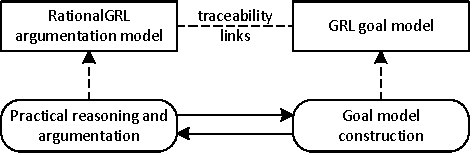
\includegraphics[width=\columnwidth]{img/framework.pdf}
\caption{The RationalGRL Framework}
\label{fig:rationalgrl-framework}
\end{figure}

\begin{table*}[t]
\centering
\begin{tabularx}{\textwidth}{|l|l|l|X|l|}
\hline
\multicolumn{2}{|c|}{\textbf{Argument scheme}} & \multicolumn{2}{c|}{\textbf{Critical Questions}} & \textbf{Effect}\\
\hline
AS0 & $a$ is an actor & CQ0 & Is the actor relevant? & \textsf{DISABLE} (no)\\
\hline
AS1 & Actor $a$ has resource $R$ & CQ1 &Is the resource available? & \textsf{DISABLE} (no)\\
\hline
AS2 & Actor $a$ can perform task $T$ & CQ2a &Is the task possible? & \textsf{DISABLE} (no)\\
&& CQ2b & Does the task have negative side-effects? & \textsf{DISABLE} (yes)\\
\hline
AS3 & Actor $a$ has goal $G$ & CQ3 & Can the desired goal be realized? & \textsf{DISABLE} (no)\\
\hline
AS4 & Actor $a$ has softgoal $S$ & CQ4 & Is the softgoal a legitimate softgoal?& \textsf{DISABLE} (no)\\
\hline
\hline
AS5 & Goal $G$ decomposes into task $T$ & CQ5a & Does the goal decompose into the task?& \textsf{DISABLE} (no)\\
& & CQ5b & Does the goal decompose into other tasks? & \textsf{INTRO} (yes)\\
 &  & CQ5c & Is the decomposition type correct? & \textsf{REPLACE} (no)\\
\hline
AS6 & Task $T$ contributes (negatively) to softgoal $S$& CQ6a & Does the task contribute to the softgoal?& \textsf{DISABLE} (no)\\
&& CQ6b & Are there alternative ways of contributing to the same softgoal?& \textsf{INTRO} (yes) \\
&& CQ6c & Does the task contribute (negatively) to some other softgoal?& \textsf{INTRO} (yes)\\
\hline
AS7 & Goal $G$ contributes to softgoal $S$ & CQ7a & Does the goal contribute to the softgoal?& \textsf{DISABLE} (no)\\
&& CQ7b & Does the goal contribute to some other softgoal?& \textsf{INTRO} (yes)\\
\hline
AS8 & Task $T$ depends on resource $R$ & CQ8 & Is the resource required in order to perform the task?& \textsf{DISABLE} (no)\\
\hline
AS9 & Actor $a$ depends on actor $b$ & CQ9 & Does the actor depend on any actors?& \textsf{INTRO} (yes)\\
\hline
AS10 & Task $T_i$ decomposes into task $T_j$ & CQ10a & Does the task decompose into the task? & \textsf{DISABLE} (no)\\
 &  & CQ10b & Does the task decompose into other tasks?& \textsf{INTRO} (yes)\\
 &  & CQ10c & Is the decomposition type correct? & \textsf{REPLACE} (no)\\
\hline
AS11 & Element $IE$ is relevant & CQ11 & Is the element relevant/useful? & \textsf{DISABLE} (no)\\
\hline
AS12 & Element $IE$ has name $n$ & CQ12 & Is the name clear/unambiguous? & \textsf{REPLACE} (no)\\
\hline
\hline
Att & Generic counterargument & Att & Generic counterargument & \textsf{DISABLE}\\
\hline
\end{tabularx}
\caption{List of argument schemes (AS0-AS13), critical questions (CQ0-CQ12), and the effect of answering them (right column).}
\label{table:argument-schemes}
\end{table*}

In the rest of this section, we discuss the individual parts of the GRL framework. In Section~\ref{sect:overview:as}, we continue our discussion of the argument schemes and critical questions for practical reasoning and argumentation, fitting these schemes and questions into our framework. In Section~\ref{sect:overview:lang}, we then discuss the language for RationalGRL models. In Section~\ref{sect:overview:examples}, we then provide extensive examples from our case study, illustrating the interplay between practical reasoning and argumentation on the one hand and RationalGRL models on the other hand.  

\subsection{The RationalGRL Argument Schemes and Critical Questions for Practical Reasoning}
\label{sect:overview:as}

A core aspect of the RationalGRL framework are the argument schemes, which should be close to the actual types of reasoning stakeholders perform (requirement 1). Recall from section \ref{sect:gmas} that we ended up with a list of argument schemes and critical questions that were found in the transcripts (Table~\ref{table:transcripts:results:argumentschemes}). Using this list as a basis, we further refined the set of argument schemes and critical questions for RationalGRL into the list shown in Table~\ref{table:argument-schemes}. Note that this list is not exhaustive, and that new argument schemes and questions can be added depending on the problem domain.

Schemes AS0-AS4 and AS12-AS13 are arguments for an element of a goal model, and AS5-AS11 are related to links in a goal model. The last scheme (Att) is a scheme for a generic counterargument against any type of argument that has been put forward. Arguments based on these schemes can be used to discuss a goal model. Making an argument based on one of the schemes effectively adds the corresponding GRL element to the model. See, for example, Table~\ref{table:transcripts:traffic-light} in Appendix~\ref{sect:transcripts:excerpts}: the participants argue for the addition of several tasks to the goal model using argument scheme AS2. 

An important part of arguing about goal models is asking the right critical questions. The critical questions presented in Table~\ref{table:argument-schemes} are therefore related to their respective argument schemes. These questions can be answered with ``yes'' or ``no'', and the type of answer has an effect on the original argument (\textsf{INTRO}, \textsf{DISABLE}, \textsf{REPLACE}). This will be further explained in Section~\ref{sect:overview:examples}. 


\subsection{The RationalGRL Modelling Language}
\label{sect:overview:lang}\label{sect:metamodel}
RationalGRL is an extension of GRL and includes all the elements shown in Figure~\ref{fig:grl_legend}. However, there are also new elements corresponding to argumentation-related concepts. Figure~\ref{fig:rationalgrllegend} shows these elements. 
\begin{itemize}
\item \emph{Argument}: This represents an argument that does not directly correspond to a GRL element.  
\item \emph{Rejected (Disabled) GRL element}: If an argument or GRL element is attacked by an argument that itself is not attacked, then this GRL element will be rejected. 
%\item \emph{Refined GRL Element}: Not all critical questions attack a GRL element. It is also possible that a critical question \emph{replaces} an existing element (for instance, by clarifying the name of the element), or that it leads to the \emph{introduction} of a new element. In these cases, the corresponding GRL element is shown with a striped background. %%Refined GRL elements are not in the metamodel and the tool also has no different picture for refined elements
\item \emph{Attack Link}: An attack link can occur between an argument and another argument or GRL element. It means that the source argument attacks the target argument or GRL element.
\end{itemize} 

\begin{figure}[b]
\centering
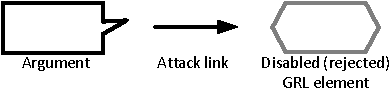
\includegraphics{img/legend.pdf}
\caption{The new elements and link of RationalGRL}
\label{fig:rationalgrllegend}
\end{figure}


The complete metamodel of the language can be found in Figure~\ref{fig:metamodel}. This metamodel represents the abstract grammar of the language, independently of the notation. The metamodel also formalizes the GRL concepts and constructs introduced in Section~\ref{sect:background:grl}.

\begin{figure*}[t]
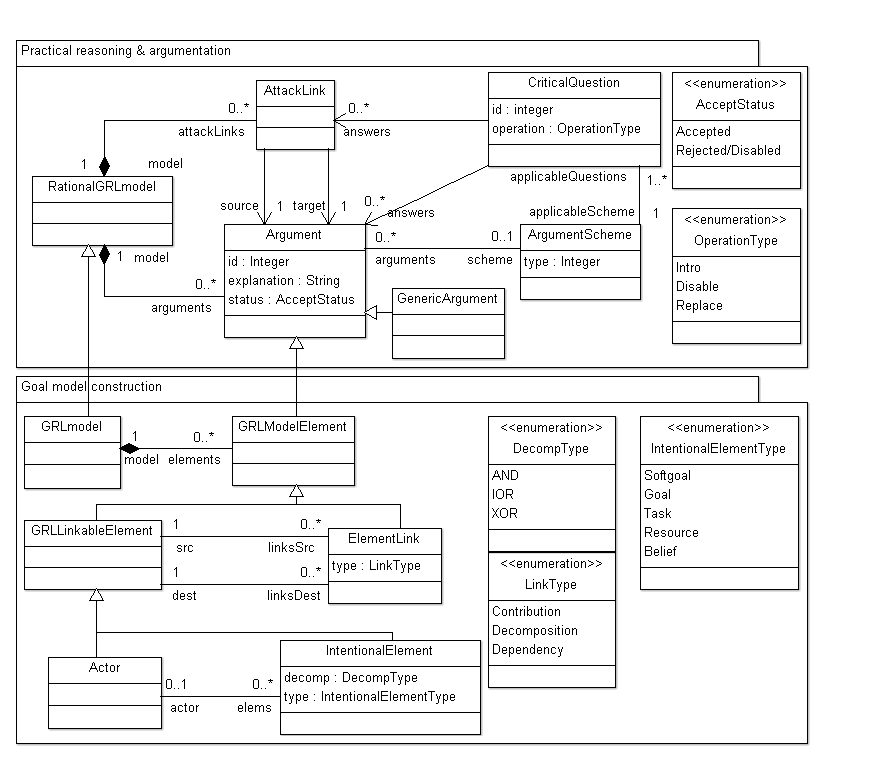
\includegraphics[width=\textwidth]{metamodel/metamodel}
\caption{The RationalGRL metamodel}
\label{fig:metamodel}
\end{figure*}

The metamodel consists of two packages, \emph{practical reasoning \& argumentation} and \emph{goal model construction}, which correspond to the relevant activities in the RationalGRL framework (cf. Figure~\ref{fig:rationalgrl-framework}). The goal model construction package consists of \textsf{GRLModelElements}, which can be either \textsf{GRLLinkableElements} or \textsf{ElementLinks}. A \textsf{GRLLinkableElement} can again be specialized into an \textsf{Actor} or an \textsf{IntentionalElement} (which is either a \textsf{Softgoal}, \textsf{Goal}, \textsf{Task}, \textsf{Resource}, or a \textsf{Belief}). Intentional elements can be part of an actor, and \textsf{GRLLinkableElements} are connected through \textsf{ElementLinks} of different types (i.e., \textsf{Contribution, Decomposition}, or \textsf{Dependency}). Finally, a \textsf{GRLmodel} is composed of \textsf{GRLModelElements}.



The practical reasoning and argumentation package depicts the concepts we introduced in Section~\ref{sect:overview:as}. An \textsf{ArgumentScheme} represents a scheme containing variables. \textsf{CriticalQuestions} are possible ways to attack or elaborate an argument based on a scheme; each critical question applies to exactly one scheme, but for each scheme there may be more than one applicable critical question. When an argument scheme is instantiated, we obtain an \textsf{Argument}. Therefore, each argument is associated with exactly one scheme, but a scheme can be instantiated in multiple ways. When a critical question is answered, we may obtain an \textsf{AttackLink}, an \textsf{Argument} or both, depending on the answer. Note that it is also possible to an \textsf{AttackLink} can also be associated with no critical questions. This allows the user to create attacks between arguments, which do not necessarily correspond to one of the critical questions. A \textsf{RationalGRLmodel} is composed out of arguments and attack relations.

Notice that there are \textsf{OperationTypes} in the Argumentation package. In RationalGRL, these operations are performed by instantiating an argument scheme or answering a critical question in a certain way. An \textsf{INTRO} operation introduces a new RationalGRL element. A \textsf{DISABLE} operation creates a new argument that attacks another argument or GRL element, effectively disabling it. The \textsf{REPLACE} operation replaces a RationalGRL element with a new element. Instantiating an argument scheme from Table~\ref{table:argument-schemes} always leads to an \textsf{INTRO} operation, that is, it always introduces a new RationalGRL element. Answering a critical question can have different effects depending on the critical question and the answer. Table~\ref{table:argument-schemes} shows these effects for the different critical questions and answers. For example, answering CQ0 with ``no'' disables the argument based on AS0. 

There are two important links between the \emph{practical reasoning \& argumentation} and \emph{goal model construction} packages. First, each \textsf{GRLModelElement} is an \textsf{Argument}. This means that each model element inherits the \textsf{AcceptStatus} as well, allowing GRL elements to be accepted or rejected. This, furthermore, means that argument schemes can be applied to all GRL elements, capturing the intuition that each GRL element can be regarded as an instantiated argument scheme. Note that besides arguments about elements of the GRL model, we also have a \textsf{GenericArgument} which is simply a counter-argument to an existing argument that does not relate to any of the GRL elements. Finally, the relation between \textsf{GRLModelElement} and \textsf{Argument} means that, as we already briefly indicated when discussing the framework in Figure~\ref{fig:rationalgrl-framework}, the class of \textsf{RatinalGRLmodel} is a superclass of \textsf{GRLmodel}: besides arguments about GRL elements, we can also have arguments that does not relate to any of the GRL elements.

\subsection{From Practical Reasoning to RationalGRL Models: examples from the case study}
\label{sect:overview:examples}

We now turn to the interactions between the \emph{practical reasoning \& argumentation} (i.e. the bottom left element of the framework in Figure~\ref{fig:rationalgrl-framework}) on the one hand, and \emph{RationalGRL models} (i.e. the top left element of the framework in Figure~\ref{fig:rationalgrl-framework}) on the other hand. We provide informal examples of the links between the practical reasoning found in our case study transcripts and RationalGRL models. The formal grounding for the connection between practical reasoning and RationalGRL models can be found in the RationalGRL Metamodel (Section~\ref{sect:metamodel}) and in more detail in the logical formalization of the Argument Schemes and Critical Questions (Section~\ref{sect:algorithms}). The connection between the RationalGRL models shown in this section and regular GRL models is further formally defined in Section \ref{sect:formalframework:translation}. 

\paragraph{Example 1 - Introducing GRL elements with arguments (\textsf{INTRO)}}

\begin{figure}[t]
\centering
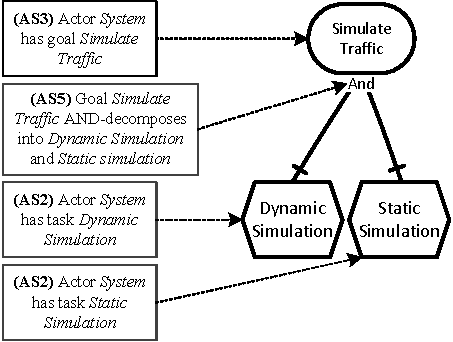
\includegraphics[width=\columnwidth]{img/fig_example_AS.pdf}
\caption{Introducing new GRL elements with argumentation (\textsf{INTRO)}.}
\label{fig:example_AS}
\end{figure}

We start by showing how instantiating argument schemes leads to the introduction of new RationalGRL elements in a model. Take the example in Figure~\ref{fig:example_AS}, which is based on the excerpt from transcript $t_1$ shown in Table~\ref{table:transcript:decomposition} in Appendix~\ref{sect:transcripts:excerpts}. On the left side, the arguments found in the transcript are shown, together with the argument scheme they are based on. The participants in the discussion argue that \emph{System} has a goal and two tasks, and that the goal AND-decomposes into the two tasks. By arguing in this way, new GRL elements are introduced. These GRL elements are shown on the right side of Figure~\ref{fig:example_AS}; the dashed arrows indicate the links between the practical reasoning and argumentation on the left and the RationalGRL model on the right. 


\paragraph{Example 2: Disabling GRL elements by answering critical questions (\textsf{DISABLE)}}

\begin{figure}[b]
\centering
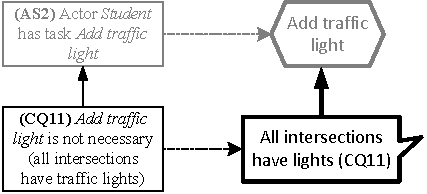
\includegraphics[]{img/fig_example_disable.pdf}
\caption{Disabling GRL tasks with argumentation (\textsf{DISABLE)}.}
\label{fig:example_disable}
\end{figure}

The excerpt from transcript $t_1$ used in this example is shown in Table~\ref{table:transcripts:traffic-light} in Appendix~\ref{sect:transcripts:excerpts}. In this example, participants first sum up functionality of the traffic simulator, which can be captured as instantiations of AS2. On left side of Figure~\ref{fig:example_disable} one such instantiation is shown, which leads to the addition of the task \emph{Add traffic light} in the RationalGRL model on the right side of Figure~\ref{fig:example_disable}. However, participant P1 notes that the problem description states that all intersections have traffic lights by default, so the task \emph{Add traffic light} is not necessary. This is captured using critical question CQ11. A negative answer to this question (cf. Table~\ref{table:argument-schemes}) should disable the original argument based on AS2 by attacking it. On the left side of Figure~\ref{fig:example_disable} a new argument (CQ11) attacks the original argument based on (AS2). This new argument is also added to the RationalGRL model on the right of Figure~\ref{fig:example_disable}, where it attacks the original task \emph{Add traffic light}. This attack leads to the original argument being \emph{rejected} (cf. Section~\ref{sect:background:pras} and Section~\ref{sect:formalframework:rationalgrl}), indicated by it being greyed out. As a result of this, the corresponding GRL task \emph{Add traffic light} is also disabled. 

\paragraph{Example 3: Changing a decomposition type by answering critical questions (\textsf{REPLACE})} 

\begin{figure}[t]
\centering
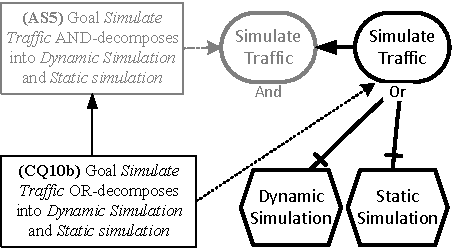
\includegraphics[]{img/fig_example_replace.pdf}
\caption{Replacing a GRL decomposition with argumentation (\textsf{REPLACE)}.}
\label{fig:examples:decomposition}
\end{figure}

The excerpt of transcript $t_3$ used for this example is shown in Table~\ref{table:transcript:decomposition} in Appendix~\ref{sect:transcripts:excerpts}. It consists of a discussion about the type of decomposition relationship for the goal \emph{Simulate Traffic} (Figure~\ref{fig:examples:decomposition}). Recall that in Example 1, an AND-decomposition was introduced for this goal with AS5 (Figure~\ref{fig:example_AS}). In the discussion CQ10b -- ``Is the decomposition type correct?'' -- is explicitly asked. The answer is ``No, it should be OR''. The original argument for AND-decomposition is now attacked  by the argument for the OR-decomposition, and the new argument is linked to the OR-decomposition in the RationalGRL model. 

\begin{figure}[b]
\centering
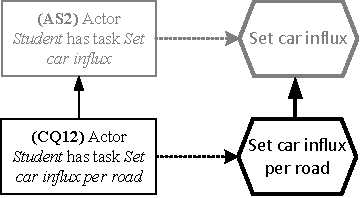
\includegraphics[]{img/fig_example_rename.pdf}
\caption{Renaming a GRL task with argumentation (\textsf{REPLACE)}.}
\label{fig:examples:clarification}
\end{figure}

\paragraph{Example 4: Clarifying a task by answering critical questions (\textsf{REPLACE})}

The transcript excerpt of this example is shown in Table~\ref{table:transcript:task-clarification} in Appendix~\ref{sect:transcripts:excerpts} and comes from transcript $t_1$. The discussion starts with an instantiation of argument scheme AS2: ``Actor \emph{Student} has task \emph{Set car influx}'' (Figure~\ref{fig:examples:clarification}). This argument is then challenged with critical question CQ12: ``Is the task \emph{Set car influx} specific enough?''. This is answered negatively, creating a new argument ``Actor \emph{Student} has task \emph{Set car influx per road}'', which attacks the original argument for \emph{Set car influx}. Note how the new task \emph{Set car influx per road} also attacks (and disables) the original RationalGRL task \emph{Set car influx}. 


\paragraph{Example 5: Defending the addition of an actor (\textsf{DISABLE)}}

\begin{figure}[t]
\centering
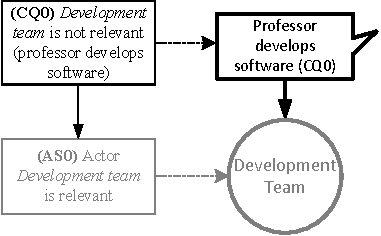
\includegraphics[]{img/reinstate1.pdf}
\caption{Disabling a GRL actor with argumentation (\textsf{DISABLE)}.}
\label{fig:examples:relevant-actor}
\end{figure}

The excerpt from transcript $t_3$ used in this example is shown in Table~\ref{table:transcript:irrelevant-actor} in Appendix~\ref{sect:transcripts:excerpts}. Actor \emph{Development Team} is introduced with an argument based on AS0 (Figure~\ref{fig:examples:relevant-actor}). This is then attacked by arguing that the professor will develop the software, so there will not be any development team (CQ0). 

\begin{figure}[b]
\centering
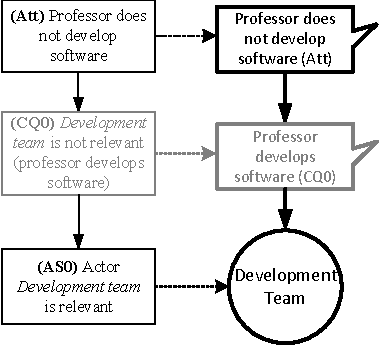
\includegraphics[]{img/reinstate2.pdf}
\caption{Defending a GRL actor by attacking its disabling attacker (\textsf{DISABLE)}.}
\label{fig:examples:relevant-actor2}
\end{figure}

Further in the discussion, it is then argued that the development team should be considered, since the professor does not develop the software. This is captured using a generic counterargument (\emph{Att}, which attacks the earlier argument based on CQ0. Figure~\ref{fig:examples:relevant-actor2} shows the situation after the counterargument has been put forward: the argument (Att) now attacks the argument (CQ0), which in turn attacks the original argument (AS0). As a result, the argument (AS0) is acceptable (cf. Section~\ref{sect:background:pras} and Section~\ref{sect:formalframework:rationalgrl}), which causes the actor in the RationalGRL model to be enabled again.


%\section{Examples}
\label{sect:gmas:examples}

We now discuss various instantiations of argument schemes and the result of answering critical questions in more detail. For each example we provide transcript excerpts, a visualization of the arguments, and the corresponding goal model elements. We provide a legend for our visualization notation in Figure~\ref{fig:legend}.

\begin{figure}[ht!]
\centering
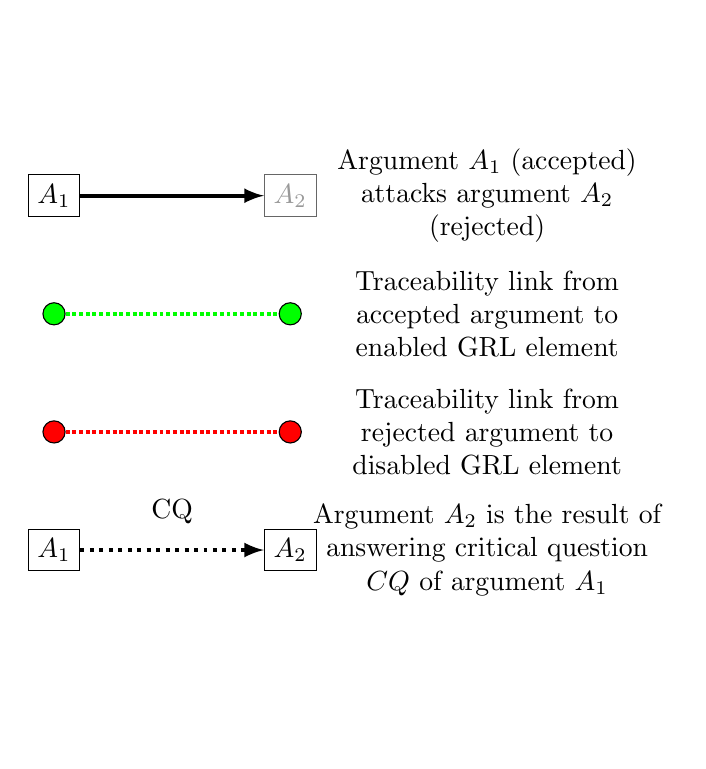
\begin{tikzpicture}
        \node (att1) [argNodeIN] at (-5,0) {$A_1$};
        \node (att2) [argNodeOUT] at (-2,0) {$A_2$};
        \node (attDescription) [draw=none, align=center] at (0.5,0) {Argument $A_1$ (accepted)\\ attacks argument $A_2$\\ (rejected)};
        \node[traceNodeGREEN] (trace1a) at (-5,-1.5) {};
        \node[traceNodeGREEN] (trace1b) at (-2,-1.5) {};
        \node (traceDescription) [draw=none,align=center] at (0.5,-1.5) {Traceability link from\\ accepted argument to\\ enabled GRL element};
        \node[traceNodeRED] (trace2a) at (-5,-3) {};
        \node[traceNodeRED] (trace2b) at (-2,-3) {};
        \node (traceDescription) [draw=none,align=center] at (0.5,-3) {Traceability link from\\ rejected argument to\\ disabled GRL element};
        \node (cq1) [argNodeIN] at (-5,-4.5) {$A_1$};
        \node (cq2) [argNodeIN] at (-2,-4.5) {$A_2$};
        \node (cqDescription) [draw=none,align=center] at (0.5,-4.5) {Argument $A_2$ is the result of\\ answering critical question\\ $CQ$ of argument $A_1$};
         \path
    (att1) edge [attackLink] (att2)
    (cq1) edge [CQLink] node [above,draw=none] {CQ} (cq2)
    (trace1a) edge[traceLinkGREEN] (trace1b)
    (trace2a) edge[traceLinkRED] (trace2b);
\end{tikzpicture}
\caption{Legend of the various elements and relationships we use for the examples in this article.}
\label{fig:legend}
\end{figure}


\subsubsection{Example 1: Disable task \texttt{Traffic light}}

The transcript excerpt of this example is shown in Table~\ref{table:transcripts:traffic-light} in the appendix and comes from transcript $t_1$. In this example, participants are summing up functionality of the traffic simulator, which are tasks that the student can perform in the simulator. All these task can be formalized and are instantiations of argument scheme AS2: ``Actor \emph{Student} has tasks $T$'', where $T\in\{$Save map, Open map, Add intersection, Remove intersection, Add road, Add traffic light$\}$''. 

Once all these tasks are summed up, participant \texttt{P1} notes that the problem description states that all intersections in the traffic simulator have traffic lights, so the task \texttt{Add traffic light} is not useful. We formalized this using the critical question CQ12: ``Is task \texttt{Add traffic light} useful/relevant?''.

We visualize some of the argument schemes, critical questions, and traceability links with the GRL model in Figure~\ref{fig:examples:traffic-light}. On the left side of the image, we see three of the instantiated argument schemes AS2. The bottom one, ``Actor \texttt{Student} has task \texttt{Add traffic light}'', is attacked by another argument generated from applying critical question CQ12: ``\texttt{Add traffic light} is useless (\emph{All intersections have traffic lights}). As a result, the corresponding GRL task is disabled. The other two tasks are enabled and have green traceability links.

\begin{figure}[ht!]
\centering
        \begin{tikzpicture}
        \node (a0) [argNodeIN] at (-2,0) {
        	\argtext{AS2}{Actor \emph{Student} has task \emph{Save map}}
        };
        \node (a1) [argNodeIN] at (-2,-2) {
        	\argtext{AS2}{Actor \emph{Student} has task \emph{Add road}}
        };
        \node (a2) [argNodeOUT] at (-2,-4) {
        	\argtext{AS2}{Actor \emph{Student} has task \emph{Add traffic light}}
        };
        \node (a3) [argNodeIN] at (-2,-6){
        	\argtext{}{\emph{Add traffic light} is useless (\emph{All intersections have traffic lights})}
        };
        \node[grl] (task1) at (2.3,0) { 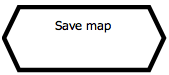
\includegraphics[scale=0.5]{img/task_save_map} };
        \node[grl] (task2) at (2.3,-2) { 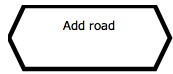
\includegraphics[scale=0.5]{img/task_add_road} };
        \node[grl, disabled] (task3) at (2.3,-4) { 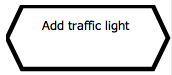
\includegraphics[scale=0.5]{img/task_add_traffic_light} };
        \node[traceNodeGREEN] (trace1a) at (-.4,-.3) {};
        \node[traceNodeGREEN] (trace1b) at (2.2,-.3) {};
        \node[traceNodeGREEN] (trace2a) at (-.4,-2.3) {};
        \node[traceNodeGREEN] (trace2b) at (2.2,-2.3) {};
        \node[traceNodeRED] (trace3a) at (-.4,-4.3) {};
        \node[traceNodeRED] (trace3b) at (2.2,-4.3) {};
         \path
    (a3) edge [attackLink] (a2)
    (a2) edge [CQLink, bend right=50] node [left,draw=none] {CQ12} (a3)
    (trace1a) edge[traceLinkGREEN] (trace1b)
    (trace2a) edge[traceLinkGREEN] (trace2b)
    (trace3a) edge[traceLinkRED] (trace3b);
\end{tikzpicture}
\caption{Argument schemes and critical questions (left), GRL model (right), and traceability link (dotted lines) for the traffic light example.}
\label{fig:examples:traffic-light}
\end{figure}


\subsubsection{Example 2: Clarify task \texttt{Road pattern}}

The transcript excerpt of the second example is shown in Table~\ref{table:transcript:task-clarification} in Appendix~\ref{sect:transcripts:excerpts} and comes from transcript $t_3$. It consists of a number of clarification steps, resulting in the task \texttt{Choose a road pattern}. 

\begin{figure}[ht!]
\centering
        \begin{tikzpicture}[->]
        \node (a0) [argNodeOUT] at (-2,0) {
        	\argtext{AS2}{Actor \emph{Student} has task \emph{Create road}}
        };
        \node (a1) [argNodeOUT] at (-2,-2) {
        	\argtext{AS2}{Actor \emph{Student} has task \emph{Choose a pattern}}
        };
        \node (a2) [argNodeOUT] at (-2,-4.2) {
        	\argtext{AS2}{Actor \emph{Student} has task \emph{Choose a pattern preference}}
        };
        \node (a3) [argNodeIN] at (-2,-6.7) {
        	\argtext{AS2}{Actor \emph{Student} has task \emph{Choose a road pattern}}
        };
        \node[grl] (actor) at (2.3,-4) { 
        	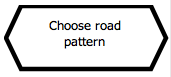
\includegraphics[scale=0.5]{img/task_choose_road_pattern} 
        };
        \node[traceNodeGREEN] (trace1) at (-.5,-7.1) {};
        \node[traceNodeGREEN] (trace2) at (2.2,-4.4) {};

\begin{pgfonlayer}{background}
         \path
    (a1) edge[attackLink] (a0)
    (a2) edge[attackLink] (a1)
    (a2) edge[attackLink, bend right=20] (a0)
    (a3) edge[attackLink] (a2)
    (a3) edge[attackLink, bend right=20] (a1)
    (a3) edge[attackLink, bend right=40] (a0);
\end{pgfonlayer}

	\path
	(a0) edge [CQLink, bend right=50] node [left,draw=none] {CQ12a} (a1)
    (a1) edge [CQLink, bend right=50] node [left,draw=none] {CQ12a} (a2)
    (a2) edge [CQLink, bend right=50] node [left,draw=none] {CQ12a} (a3)
    (trace1) edge[traceLinkGREEN] (trace2);
\end{tikzpicture}
\caption{Argument schemes and critical questions (left), GRL model (right), and traceability link (dotted line) of the road pattern example.}
\label{fig:examples:clarification}
\end{figure}

The formalized argument schemes and critical questions are shown in Figure~\ref{fig:examples:clarification}. The discussion starts with the first instantiation of argument scheme AS2: ``Actor \texttt{Student} has task \texttt{Create road}''. This argument is then challenged with critical question CQ12: ``Is the task \texttt{Create road} clear?''. Answering this question results in a new instantiation of argument scheme AS2: ``Actor \texttt{Student} has task \texttt{Choose a pattern}''. This process is repeated two more times, resulting in the final argument ``Actor \texttt{Student} has task \texttt{Choose a road pattern}''. This final argument is unattacked and has a corresponding intentional element (right image). 

What is clearly shown in this example is that a clarifying argument attacks all arguments previously used to describe the element. For instance, the final argument on the bottom of Figure~\ref{fig:examples:clarification} attacks all three other arguments for a name of the element. If this was not the case, then it may occur that a previous argument is \emph{reinstatiated}, meaning that it becomes accepted again because the argument attacking it is itself attacked. Suppose for instance the bottom argument ``Actor \texttt{Student} has task \texttt{Choose a pattern preference}'' did not attack the second argument: ``Action \texttt{Student} has task \texttt{Choose a pattern}''. In that case, this argument would be reinstated, because its only attacker ``Actor \texttt{Student} has task \texttt{Choose a pattern preference}'' is itself defeated by the bottom argument.

\subsubsection{Example 3: Decompose goal \texttt{Simulate}}

The transcript excerpt of this example is shown in Table~\ref{table:transcript:decomposition} in the appendix and comes from transcript $t_3$. It consists of a discussion about the type of decomposition relationship for the goal \texttt{Simulate}.

\begin{figure}[ht!]
\centering
        \begin{tikzpicture}[->]
        \node (a0) [argNodeIN] at (-2,0) {
        	\argtext{AS3}{Actor \emph{System} has goal \emph{Simulate}}
        };
        \node (a1) [argNodeIN] at (-2,-1.5) {
        	\argtext{AS2}{Actor \emph{System} has task \emph{Dynamic simulation}}
        };
        \node (a2) [argNodeIN] at (-2,-3) {
        	\argtext{AS2}{Actor \emph{System} has task \emph{Static simulation}}
        };
        \node (a3) [argNodeOUT] at (-2,-5) {
        	\argtext{AS5}{Goal \emph{Simulate} AND-decomposes into \emph{Static simulation} and \emph{Dynamic simulation}}
        };
        \node (a4) [argNodeIN] at (-2,-7.5) {
        	\argtext{AS5}{Goal \emph{Simulate} OR-decomposes into \emph{Static simulation} and \emph{Dynamic simulation}}
        };
        \node[grl] (actor) at (2.3,-4) { 
        	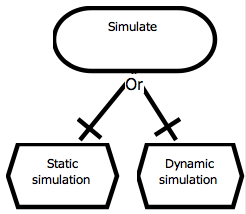
\includegraphics[scale=0.5]{img/simulate_decomposition} 
        };
        \node[traceNodeGREEN] (trace1a) at (-.4,-.3) {};
        \node[traceNodeGREEN] (trace1b) at (2.5,-3.1) {};
        \node[traceNodeGREEN] (trace2a) at (-.4,-1.8) {};
        \node[traceNodeGREEN] (trace2b) at (3.5,-5.6) {};
        \node[traceNodeGREEN] (trace3a) at (-.4,-3.3) {};
        \node[traceNodeGREEN] (trace3b) at (1.3,-5.6) {};
        \node[traceNodeGREEN] (trace4a) at (-.4,-8.2) {};
        \node[traceNodeGREEN] (trace4b) at (2.5,-3.9) {};

\begin{pgfonlayer}{background}
         \path
    (a4) edge[attackLink] (a3);
\end{pgfonlayer}

	\path
	(a3) edge [CQLink, bend right=50] node [left,draw=none] {CQ10b} (a4)
    (trace1a) edge[traceLinkGREEN] (trace1b)
    (trace2a) edge[traceLinkGREEN] (trace2b)
    (trace3a) edge[traceLinkGREEN] (trace3b)
    (trace4a) edge[traceLinkGREEN, bend right] (trace4b);
\end{tikzpicture}
\caption{Argument schemes and critical questions (left), GRL model (right), and traceability link (dotted line) of the goal decomposition example.}
\label{fig:examples:decomposition}
\end{figure}

The visualization of this discussion is shown in Figure~\ref{fig:examples:decomposition}. Each GRL element on the right has a corresponding argument on the left. Moreover, the original argument for an AND-decomposition is attacked by the argument for the OR-decomposition, and the new argument is linked to the decomposition relation in the GRL model.

\subsubsection{Example 4: Reinstate actor \texttt{Development team}}

The transcript excerpt of this example is shown in Table~\ref{table:transcript:irrelevant-actor} in the appendix and comes from transcript $t_3$. It consists of two parts: first participant \texttt{P1} puts forth the suggestion to include actor \texttt{Development team} in the model. This is, then, questioned by participant \texttt{P2}, who argues that the professor will develop the software, so there won't be any development team. However, in the second part, participant \texttt{P2} argue that the development team should be considered, since the professor does not develop the software.

\begin{figure}[ht!]
\centering
        \begin{tikzpicture}
        \node (a0) [argNodeOUT] at (-2,0) {
        	\argtext{AS0}{Development team is relevant}
        } ;
        \node (a1) [argNodeIN] at (-2,-2.5){
        	\argtext{}{Development team is not relevant (\emph{The professor makes the software})}
        };
        \node[grl, disabled] (actor) at (2.3,-1) { 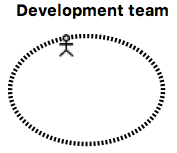
\includegraphics[scale=0.5]{img/actor_development_team} };
        \node[traceNodeRED] (trace1) at (-.5,-.3) {};
        \node[traceNodeRED] (trace2) at (2.2,-0.1) {};

         \path
    (a1) edge[attackLink] (a0)
    (a0) edge [CQLink, bend right=50] node [left,draw=none] {CQ0} (a1)
    (trace1) edge[traceLinkRED] (trace2);
\end{tikzpicture}
\caption{Argument schemes and critical questions (left), GRL model (right), and traceability link (dotted line) of a discussion about the relevance of actor Development team.}
\label{fig:examples:relevant-actor}
\end{figure}

We formalize this using a \emph{generic counterargument}, attacking the critical question. The first part of the discussion is shown in Figure~\ref{fig:examples:relevant-actor}. We formalize the first statement as an instantiation of argument scheme AS0: ``Actor \texttt{development team} is relevant''. This argument is, then, attacked by answering critical question CQ0: ``Is actor \texttt{development team} relevant? with \emph{No}. This results in two arguments, AS0 and CQ0, where CQ0 attacks AS0. This is shown in Figure~\ref{fig:examples:relevant-actor}, left image.

\begin{figure}[ht!]
\centering
        \begin{tikzpicture}
        \node (a0) [argNodeIN] at (-2,0) {
        	\argtext{AS0}{Development team is relevant}
        };
        \node (a1) [argNodeOUT] at (-2,-2.5){
        	\argtext{}{Development team is not relevant (\emph{The professor makes the software})}
        };
        \node (a2) [argNodeIN] at (-2,-5) {
        	\argtext{}{The professor doesn't develop the software}
        } ;
        \node[grl] (actor) at (2.3,-1) { 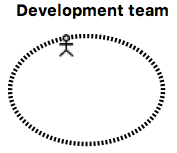
\includegraphics[scale=0.5]{img/actor_development_team} };
        \node[traceNodeGREEN] (trace1) at (-.5,-.3) {};
        \node[traceNodeGREEN] (trace2) at (2.2,-0.1) {};

         \path
    (a1) edge[attackLink] (a0)
    (a2) edge[attackLink] (a1)
    (a0) edge [CQLink, bend right=50] node [left,draw=none] {CQ0} (a1)
    (a1) edge [CQLink, bend right=50] node [left,draw=none] {Att} (a2)
    (trace1) edge[traceLinkGREEN] (trace2);
\end{tikzpicture}
\caption{Argument schemes and critical questions (left), GRL model (right), and traceability link (dotted line) of a discussion about the relevance of actor Development team.}
\label{fig:examples:relevant-actor2}
\end{figure}

Figure~\ref{fig:examples:relevant-actor2} shows the situation after the counter argument has been put forward. The argument ``Actor \texttt{Professor} doesn't develop the software'' now attacks the argument ``\texttt{Development team} is not relevant (\emph{The professor makes the software})'', which in turn attacks the original argument ``\texttt{Development team} is relevant''. As a result, the first argument is reinstated, which causes the actor in the GRL model to be enabled again.
\section{The RationalGRL Methodology and Tool}
\label{sect:methodology}

In previous sections, we have shown how the RationalGRL framework can capture stakeholder discussions, and how interactions between two types of reasoning, practical reasoning and goal modeling, leads to two interlinked models, RationalGRL and GRL models. In this section we clarify how practitioners can actually use the RationalGRL framework by proposing a methodology (\textbf{requirement 4}) and discussing a prototype RationalGRL tool (\textbf{requirement 5}).

\subsection{RationalGRL Methodology}
\label{sect:methodology} 

We propose the methodology shown in Figure~\ref{fig:rationalgrl-methodology} to develop a (Rational)GRL model, an earlier version of which was presented at the 2017 iStar workshop \cite{ghanavatiMethodology}. %Here we assume that the initial GRL models have been created based on the requirements specification documents and the discussions of the stakeholders. The rest of the steps are as follows:

\textbf{(1) Instantiate Argument Schemes (AS)} -- We start with the list of argument schemes (Table~\ref{table:argument-schemes}). Whilst discussing the requirements, we select schemes from the list and instantiate them to form arguments for GRL model elements. In this way we build or modify the GRL model by introducing new GRL elements (\textsf{INTRO}). Note that it is also possible to start modifying an existing GRL model which was not built using the RationalGRL methodology: each GRL element corresponds to an argument (i.e. an instantiated scheme), so it is possible to instantiate argument schemes based on an existing GRL model. 

\textbf{(2) Answer Critical Questions (CQs)} -- After building or modifying the initial GRL model, we ask the relevant critical questions. Because each element in the GRL model corresponds to an instantiated scheme, we can look at Table~\ref{table:argument-schemes}) to see which questions are relevant given our GRL model. 

\textbf{(3) Decide on Intentional Elements and their Relationships} -- By answering a critical question, one of the \textsf{INTRO}, \textsf{DISABLE} or \textsf{REPLACE} are performed on the GRL model. Any of these operations impact the arguments and corresponding GRL intentional elements, modifying the initial GRL model into a RationalGRL model. After these modifications, we can keep on asking critical questions (e.g. about elements that were introduced by previously answering a critical question) until we are satisfied with our model.   

\textbf{(4) Modify GRL Models} -- Based on the RationalGRL model of step (3), the GRL model can be modified: 1) a new intentional element or a new link is introduced; 2) an existing intentional element or an existing link gets disabled (removed) from the model; or 3) an existing intentional element or link is replaced by a new one. This results in a new, modified GRL model, which can be used as the basis for another cycle of the methodology. 

We can continue these four steps until there is no more intentional element or link to analyze or we reach a satisfactory model. In the next section, we will give an example of how our tool can be used together with the methodology to build a GRL model.  

\begin{figure*}[t]
\centering
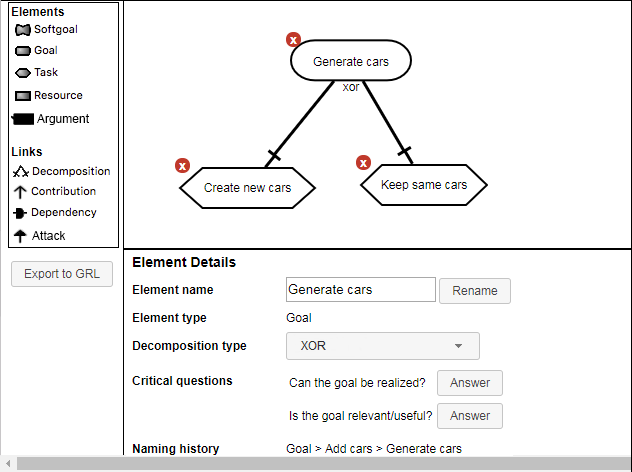
\includegraphics[scale=0.8]{img/tool/goal_details}
\caption{Overview of the RationalGRL tool}
\label{fig:tool:overview}
\end{figure*}


\subsection{The RationalGRL Tool}
\label{sect:tool}

An important requirement of our framework is that it has tool support (\textbf{requirement 5}. This is for various reasons: i) although there are various approaches attempting to combine goal modeling with argumentation, there does not yet exist any tool support (see Section~\ref{sect:discussion}), ii) it allows us to do user tests in future research, exploring the difference between GRL and RationalGRL, iii) tool support is an excellent verification to ensure our formal framework and algorithms actually work, iv) having a light-weight web-based version of GRL is useful for the community in general. In this section we briefly highlight some features of the tool, and we explain some of its current limitations.

GRL has a well-documented and well-maintained tool called jUCMNav~\cite{jUCMNav}\footnote{\url{http://jucmnav.softwareengineering.ca/foswiki/ProjetSEG}}, which is implemented as an Eclipse plugin. Although it is a rich tool with many features, it can take significant time to set it up properly and is quite feature-heavy. Therefore, we have decided to implement our own lightweight modelling tool as our proof-of-concept. The tool can be accessed from:

\begin{quote}
\url{http://www.rationalgrl.com}
\end{quote}

The RationalGRL tool is an open-source\footnote{\url{http://www.github.com/marcvanzee/RationalGRL}}, web-based Javascript application, which runs on all modern browsers. The tool is based on our formalization in Section~\ref{sect:formalframework}. Because this formalization is very close to the GRL metamodel, the models can be easily exported to jUCMNav.

When the tool starts, the user is presented with a screen as in Figure~\ref{fig:tool:overview}. This screen shows the palette of elements and links to the left, a canvas on which RationalGRL models can be built, and a pane with details of the currently selected elements on the canvas. Elements and links can be added to the canvas by selecting them on the left and clicking on the canvas, thus capturing the \textsf{INTRO} operation (Section~\ref{sect:formalframework:intro}). This makes it possible to build and modify regular GRL models using the tool. 

The details panel can be used to answer the critical questions of the RationalGRL framework (Table~\ref{table:argument-schemes}): Figure~\ref{fig:tool:overview}, for example, shows two critical questions for the goal element ``Generate cars'', namely ``Can the goal be realized?'' (CQ3) and ``Is the goal relevant/useful?'' (CQ11). Clicking the ``Answer'' button next to a critical question allows the user to answer the question. As an example, consider Figure~\ref{fig:tool:cqdetails}, where the softgoal ``Easy to use'' is questioned with the relevancy question (CQ11). It is possible to select the answer and provide an explanation for the answer. 

Assume that in the example of Figure~\ref{fig:tool:cqdetails} the user selects ``No'' and clicks the ``Answer question'' button. A new argument is then automatically created that attacks the softgoal and the details pane shows the critical question as answered (Figure~\ref{fig:tool:cqeffect}). This is an implementation of a \textsf{DISABLE} algorithm (Section~\ref{sect:formalframework:disable}) similar to Algorithm~\ref{alg:actor-not-relevant}: a new argument is added that attacks the existing argument. It is also possible to attack arguments by adding an ``Argument'' element and an ``Attack'' link manually. Consider, for example, Figure~\ref{fig:tool:argument}. Here, a new argument ``Necessary'', which attacks the previously generated argument based on CQ11, has been added by the user. As the details pane shows, this new argument is not based on a CQ. It is further worth noting that it is possible to provide further a explanation in argument elements, allowing for more fine-grained rationalizations. 

\begin{figure}[t]
\centering
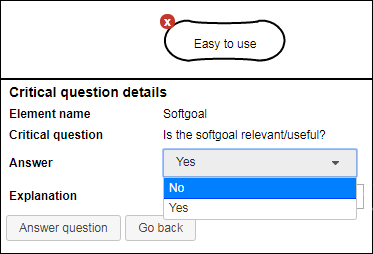
\includegraphics[width=0.8\columnwidth]{img/tool/details_softgoal}
\caption{Critical question details pane for ``Is the softgoal relevant/useful?''}
\label{fig:tool:cqdetails}
\end{figure}

\begin{figure}[b]
\centering
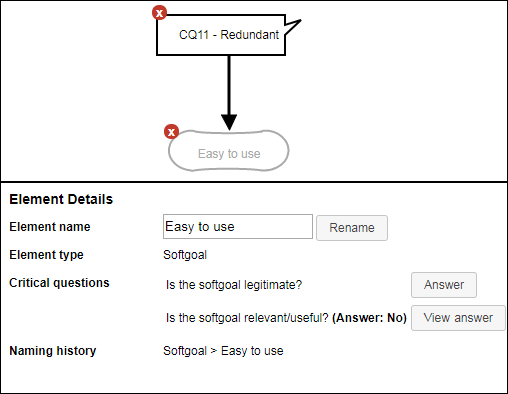
\includegraphics[width=\columnwidth]{img/tool/attack_softgoal}
\caption{Effect of answering CQ11: ``Is the softgoal relevant/useful?'' with ``No''}
\label{fig:tool:cqeffect}
\end{figure}

The RationalGRL tool computes the acceptability of arguments on the fly. In the example of Figure~\ref{fig:tool:cqeffect}, the original (argument for) softgoal ``Easy to use'' is rejected because it's only attacker ``CQ11 - Redundant'' is accepted. However, if we then attack ``CQ11 - Redundant'' with a new argument ``Necessary'', the original argument for ``Easy to use'' is again accepted because its only attacker is rejected  (Figure~\ref{fig:tool:argument}). Note that when computing the acceptability of arguments, the RationalGRL tool makes the assumption that there are no attack cycles in the model and that hence there is one unique preferred extension (cf. Section~\ref{sect:formalframework:rationalgrl}) -- if the user creates an attack cycle, an error message is shown. 

\begin{figure}[t]
\centering
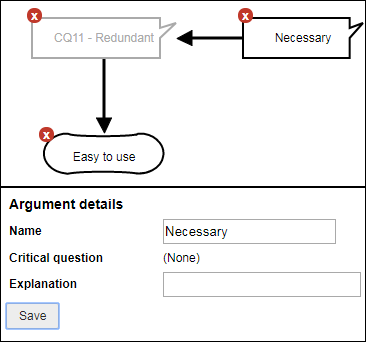
\includegraphics[width=0.8\columnwidth]{img/tool/reinstate_softgoal}
\caption{Attacking an argument with a generic argument ``Necessary''}
\label{fig:tool:argument}
\end{figure}

The final operation that has been captured in the RationalGRL tool is \textsf{REPLACE}. For usability purposes, this operation has been implemented differently than in our formal framework (Section~\ref{sect:formalframework:disable}). In the formal framework, a \textsf{REPLACE} introduces a new argument that replaces (and therefore attacks) all previous arguments with the same identifier. Including \textsf{REPLACE} like this in the tool would mean that, when the name of an element is changed, we would need to render all the previous versions of the element on the canvas of the tool. Because this would quickly become very cumbersome, we decided to implement a naming history for each element. For example, in Figure~\ref{fig:tool:overview}, the goal ``Generate cars'' was previously named ``Add cars''. In this way, a history is kept of how an element name was clarified without cluttering the model canvas. Similarly, the decomposition type can be changed in the details pane (Figure~\ref{fig:tool:overview}) without introducing new elements that attack the original ones (cf. Figure~\ref{fig:example-small3}, where the old decomposition type $AND$ of ``Generate traffic'' is shown as an explicit argument).  

The tool further implements the RationalGRL to GRL translation (Algorithm~\ref{alg:translation:to-grl}) through an export function. RationalGRL models built in the RationalGRL tool can be exported to the \texttt{.grl} file format, which can be imported in jUCMNav. Two examples of this export are provided in Appendix~\ref{sect:tool-screenshots}. Figure~\ref{fig:tool:figfrompaper} shows the model that was discussed earlier in this paper (Figure~\ref{fig:example-small3}) in the RationalGRL tool. Recall that translating this model to GRL provided us with the model in Figure~\ref{fig:example-small}. This is also what follows from our export: if we export the RationalGRL model and then import the resulting GRL model in jUCMNav, we get the model in Figure~\ref{fig:tool:figfrompaper1}, which is the same as Figure~\ref{fig:example-small}.

Our translation and export function uses the argument acceptability as a way of determining the GRL model. Take for example, the RationalGRL model in Figure~\ref{fig:tool:multipleattack}. A positive contribution is added from ``Keep same cars'' to ``Simple design''. More inportantly, an argument ``not enough CPU'' has been added to the model. This argument attacks the ``Realistic simulation'' softgoal and the ``Create new cars'' task, arguing that there is not enough processing power for either of these to be feasible in the traffic simulator. Now, if we export this to GRL, the GRL elements that are rejected or disabled (greyed out in Figure~\ref{fig:tool:multipleattack}) are not included. This can be seen in Figure~\ref{fig:tool:multipleattack1}, where the jUCMNav GRL model that was exported from the RationalGRL tool is shown. The pair of figures \ref{fig:tool:multipleattack} and \ref{fig:tool:multipleattack1} also nicely shows the added value of RationalGRL: Figure~\ref{fig:tool:multipleattack} shows that there can be a larger discussion and rationalization underlying even a fairly simple goal model such as the one in Figure~\ref{fig:tool:multipleattack1}. 

   

 

\section{RationalGRL: Logical Framework}
\label{sect:formalframework}

In Section~\ref{sect:overview}, we have shown through a language definition and informal examples from our case study that it is possible to trace elements of the goal model back to their underlying arguments (requirement 2), and that it is possible to determine the effect of changes in the underlying argumentation on the goal model, and vice versa (requirement 3). A more formal, logical rendition of this traceability will be presented in this section. Our main approach here is to use formal argumentation, which allows us to use many of the techniques developed in that area directly (see Section~\ref{sect:background:pras}).

In Section~\ref{sect:goalmodeling:logicallanguage} we present the basic logical language of our formalism, based on the metamodel from Section~\ref{sect:overview:lang}. Section~\ref{sect:goalmodeling:argumentationsemantics} then presents formal definitions of arguments and how the status of arguments can be computed, which was already briefly informally discussed in Section~\ref{sect:background:pras}. In Section~\ref{sect:algorithms} we then develop algorithms for instantiating argument schemes and for answering critical questions, formally capturing the \textsf{INTRO}, \textsf{REPLACE} and \textsf{DISABLE} operations of which examples were previously given in Section~\ref{sect:overview:examples}. Finally, in Section~\ref{sect:rationalGRL-GRL} we define the link between RationalGRL models on the one hand and GRL models -- which form a subset of the set of RationalGRL models -- on the other hand, formally capturing the export function of our tool (cf. Section~\ref{sect:tool}). 

\subsection{Logical Language for RationalGRL}
\label{sect:goalmodeling:logicallanguage}

We assume familiarity with basic notions from propositional logic and set theory. An \emph{atom} is a formula with no logical connectives ($\vee, \wedge, \rightarrow, \leftrightarrow$) or negation ($\neg$).  A \emph{ground atom} is an atom without variables.

We first define the logical language for RationalGRL. This logical language is largely based on the metamodel (Section~\ref{sect:overview:lang}).

\begin{definition}[RationalGRL Language]
The \emph{RationalGRL language} $\mathcal{L}$ contains the following atoms:
\begin{itemize}
\item $actor(i,n)$: Identifier $i$ is an actor with name $n$.
\item $IE(i,n,t,dt)$: Element with identifier $i$ is an intentional element with name $n$ of type $t$ and with decomposition-type $dt$, where: 
\begin{itemize}
\item $t$ is one of $softgoal$, $goal$, $task$, $resource$ or $belief$
\item $dt$ is one of $and$, $or$, $xor$ or $none$.
\end{itemize}
\item $EL(k,i,j,lt)$: The element link with identifier $k$ is of link-type $lt$ and links the element with identifier $i$ to the element with identifier $j$, where:
\begin{itemize}
\item $t$ is one of $decomposition$, $dependency$ or $contribution$
\end{itemize}
\item $has(i,j)$: Identifier $i$ (which is an actor) has the element corresponding to identifier $j$.
\item $arg(i,n)$: Element with identifier $i$ is a generic argument with name $n$
\item $disable(i,r)$: The element or relationships corresponding to identifier $i$ should be disabled because reason $r$.
\end{itemize}

\noindent Identifiers $i,j,k$ are natural numbers. Names $n$, types $t, dt, lt$ and reasons $r$ are strings. We assume that links and elements have unique identifiers and names. 
\end{definition}

\todo{F}{M}{Ik ben niet helemaal gelukkig met IE en EL. Ik had eerst $intentional\_element(i,n,t,dt)$ en $element\_link(k,i,j,lt)$ maar dat komt slecht uit in voorbeelden en algoritmes omdat dat lange namen zijn. Wat vind jij?}

Using the language from Definition 1, we can define GRL models.

\begin{definition}[GRL model] \label{def:rationaGRLmodel}
A \emph{GRL model} $\mathcal{M}$ is a set of ground atoms based on $\mathcal{L}$, without atoms of the form $arg(i,n)$ and $disable(i,r)$.
\end{definition}

An example of the specification of the RationalGRL model in Figure~\ref{fig:example_AS} is shown in Table~\ref{table:grl_atom_spec}, written in logic programming style. A more elaborate example of a specification is shown in Appendix~\ref{ch:grlspec}, showing a complete specification of the traffic simulator GRL model in Figure~\ref{fig:trafficsim}\todo{F}{M}{change Appendix specification to match the still-to-be-created example in section~\ref{sect:tool}}.

Notice that Definition~\ref{def:rationaGRLmodel} does not put any constraints on a RationalGRL model. If desired, constraints can be captured using simple axioms which enforce, for example, that each element link has one source and one destination element, both of which are intentional elements. For simplicity's sake, we will leave these constraints implicit in this article. 

\begin{table}[h!]
\centering
\begin{tabularx}{\columnwidth}{|X|}
\hline
\texttt{actor(0,system).}\\
\texttt{IE(1,simulate\_traffic, goal, or).}\\
\texttt{IE(2,static\_simulation, task, none).}\\
\texttt{IE(3,dynamic\_simulation, task, none).}\\
\texttt{has(0,1).}\\ 
\texttt{has(0,2).}\\ 
\texttt{has(0,3).}\\
\texttt{EL(4,2,1,decomposition).}\\
\texttt{EL(5,3,1,decomposition).}\\

\hline
\end{tabularx}
\caption{Specification of the RationalGRL model in Figure~\ref{fig:example_AS}}
\label{table:grl_atom_spec}
\end{table}

\subsection{Formal argumentation}
\label{sect:goalmodeling:argumentationsemantics}

In the previous subsection we introduced a language to specify a RationalGRL model. In this subsection we give a formal definition of an argument.

\begin{definition}[Argument] \label{def:argument}
An \emph{argument} $A\subseteq Args$ is a set of ground atoms based on $\mathcal{L}$.
\end{definition}

This simple definition allows us to form arguments about (parts of) a RationalGRL model. For instance, $A_1$: $\{actor(0,system)\}$ is an argument stating that there is an actor \emph{system}, $A_2$: $IE(1,goal,simulate\_traffic,none)$ is an argument stating that there is a goal \emph{simulate\_traffic}, $A_3$: $\{has(0,1)\}$ is an argument stating that the actor with id $0$ (in this case \emph{system}) has has goal \emph{simulate\_traffic}, and $A_4 = A_1 \cup A_2 \cup A_3$ is one argument for the fact that actor \emph{system} has goal \emph{simulate\_traffic}. 

Note that, like a RationalGRL model, an argument is a set of atoms from our language. This makes sense: as the metamodel (Figure~\ref{fig:metamodel}) shows, a RationalGRL model is comprised of arguments, that is, it is the union of all arguments. Furthermore, similar to Definition~\ref{def:rationaGRLmodel} for RationalGRL models, Definition~\ref{def:argument} does not put any restrictions on the content of an argument, which makes it possible to form arguments that do not correspond to correct or sensible RationalGRL models. For example, argument $A_3$ from the above example only makes sense if there is an actor with id $0$ and an intentional element with id $1$. While we could have chosen to put logical constraints on the content of an argument, we choose not to do so here. Instead, we put these restrictions on the algorithms in section~\ref{sect:algorithms}. The algorithms are constructed in such a way that they only allow the construction of arguments that correspond to valid RationalGRL models. The advantage of this approach is that it keeps the presentation of the formal part relatively simple.

In line with the main approaches in formal argumentation, we next introduce an argumentation framework as a set of arguments and an attack relation between the arguments.

\begin{definition}[Argumentation framework~\cite{Dung1995}] \label{def:argumentationframework}
An argumentation framework $AF=(Args,Att)$ consists of a set of arguments $Args$ and an attack relationship $Att:Args\times Args$, where $(A_1,A_2)\in Att$ means that argument $A_1\in Args$ attacks arguments $A_2\in Args$.
\end{definition}

In order to determine which arguments are accepted or not, we define \emph{argumentation semantics}. 

\begin{definition}[Argumentation Semantics] Suppose an argumentation framework $AF=(Arg,Att)$, two sets of arguments $S\cup S'\subseteq Arg$, and some argument $A\in Arg$. We say that
\begin{itemize}
\item $S$ \emph{attacks} $A$ if some argument in $S$ attacks $A$,
\item $S$ \emph{attacks} $S'$ if some argument in $S$ attacks some argument in $S'$,
\item $S$ is \emph{conflict-free} if it does not attack itself,
\item $S$ \emph{defends} $A$ if for each $B$ such that $B$ attacks $A$, $S$ attacks $B$,
\item $S$ is \emph{admissible} if $S$ is conflict-free and defends each argument in it.
\item $S$ is a \emph{preferred extension} of $AF$ if $S$ is a maximal (w.r.t. set inclusion) admissible set of $AF$.
\end{itemize}
\end{definition}

\begin{figure}[ht!]
\centering
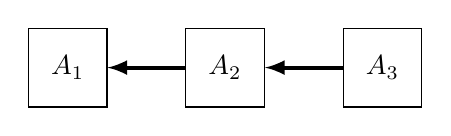
\begin{tikzpicture}
        \node[minimum size=1cm] (b) [argNodeIN] at (-2,0) {$A_1$};
        \node[minimum size=1cm] (c) [argNodeIN] at (0,0) {$A_2$};
        \node[minimum size=1cm] (d) [argNodeIN] at (2,0) {$A_3$};
             
         \path
    (c) edge [attackLink] (b)
    (d) edge [attackLink] (c);
    
\end{tikzpicture}
\caption{Example argumentation framework.}
\label{fig:goalmodeling:arg2}
\end{figure}

Let us explain these definitions using the example argumentation framework in Figure~\ref{fig:goalmodeling:arg2}, where $A_2$ attacks $A_1$ and $A_3$ attacks $A_2$. There are two admissible sets: $\{A_3\}$ and $\{A_1, A_3\}$, in which $A_3$ defends $A_1$ against its attacker $A_2$. Sets containing both $A_2$ and either $A_1$ or $A_3$ are not conflict free, and the sets $\{A_1\}$ and $\{A_2\}$ do not defend themselves against $A_2$ and $A_3$, respectively. Given the notion of admissible sets, we can then define our extensions. There are a large number of different semantics to determine which arguments are in an extension; in this article, we choose preferred semantics. In our example from Figure~\ref{fig:goalmodeling:arg2}, there is one preferred extension, namely $\{A_1,A_3\}$. Based on this extension, we can define the status of arguments, acceptable or rejected. 

\begin{definition}[Acceptable and Rejected Arguments] Given an argumentation framework $AF=(Arg,Att)$, an argument $A$ is \emph{acceptable} if $A$ is in the preferred extension of $AF$, and rejected otherwise. 
\end{definition}

This means that, given the argumentation framework in Figure~\ref{fig:goalmodeling:arg2}, arguments $A_1$ and $A_3$ are acceptable and $A_2$ is rejected.

\subsection{Algorithms for argument schemes and critical questions}
\label{sect:algorithms}

In Section~\ref{sect:goalmodeling:logicallanguage} we have developed a simple logical language with which to capture RationalGRL models. We then (Secton~\ref{sect:goalmodeling:argumentationsemantics} formalized an argument as a set of atoms from our language, and we introduced \emph{argumentation semantics} to compute sets of accepted arguments. In this section we develop algorithms for applying argument schemes and critical questions. These algorithms define which arguments should be introduced whenever an argument scheme is instantiated or a critical question is answered. In other words, the algorithms define the exact application of the \textsf{INTRO}, \textsf{REPLACE} and \textsf{DISABLE} operations for the different argument schemes and critical questions. The arguments and attack relations produced by the algorithms then together form an argumentation framework with an associated preferred extension, which can be interpreted as a RationalGRL model. 

\subsubsection*{Algorithms for argument schemes}

In the following algorithms, $id$ is the current highest identifier of the elements, which is increased for each new element that is added, $Args$ is the set of all arguments and $Att$is the set of all attack relations. 

The algorithms for the argument schemes consist of forming a new argument and adding it to the set of arguments. No attack relations are introduced.

\begin{algorithm}[h]
  \caption{Applying AS0: Actor $n_{a}$ is relevant}\label{alg:as0}
  \begin{algorithmic}[1]
    \Procedure{$AS_0$}{$n_{a}$}
    \State $id\gets id+1$\label{alg:as0:1}
    \State $A \gets \{actor(id, n_{a})\}$\label{alg:as0:2}
    \State $Args \gets Args \cup A$\label{alg:as0:3}
    \EndProcedure
  \end{algorithmic}
\end{algorithm}

\noindent\textbf{Algorithm~\ref{alg:as0} for argument scheme AS0}: The algorithm takes one argument, namely the name $n_{a}$ of the actor. On line~\ref{alg:as0:1} of the algorithm, the global variable $id$ is increased by one. This ensures that each new argument has a unique identifier. 
On line~\ref{alg:as0:2}, the argument for the actor is formed consisting of the statement that there is an actor with $id$ and name $n_{a}$ and on line~\ref{alg:as0:3} this argument is added to the set of arguments $Args$. In Figure~\ref{fig:examples:relevant-actor2}, the application of the argument scheme $AS_0(\text{Development team})$, results in one argument: $\{actor(0, \text{Development team})\}$.

\begin{algorithm}[h]
  \caption{Applying AS1-AS4: Actor $id_{a}$ has intentional element $n_{ie}$ of type $t_{ie}$}\label{alg:as1}
  \begin{algorithmic}[1]
    \Procedure{$AS_1$}{$id_{a}$, $n_{ie}$, $t_{ie}$}
    \State $id\gets id+1$
    \State $A\gets \{IE(id,n_{ie},t_{ie},none), has(id_{a},id)\}$
    \State $Args \gets Args\cup A$
    \EndProcedure
  \end{algorithmic}
\end{algorithm}
\todo{F}{M}{fix tekst bij aangepast algoritme}
\noindent\textbf{Algorithm~\ref{alg:as1} for argument scheme AS1:} This argument scheme takes two arguments, the identifier $a_{id}$ of the actor and the resource name $n$. The algorithm is similar to the previous one, with the difference that the newly added argument contains the statement $has(a_{id},id)$ as well, meaning that the actor with id $a_{id}$ has element $id$ (which is a resource). As an example, let us formalize the argument corresponding to resource \emph{External library} of actor \emph{Traffic tycoon} in Figure~\ref{fig:transcripts:grl}. First, we assume some id is associated with the actor: $$\{actor(0),name(0,traffic\_tycoon)\}.$$ Then we can formalize the argument for the resource as follows: $$\{resource(1),name(1,external\_library),has(0,1)\}.$$

Argument scheme AS1 to AS4 are all very similar, in the sense that they all assert that some element belongs to an actor. Therefore, we only provide the algorithm for AS1 and we assume the reader can easily construct the remaining algorithms AS2-AS4.

\begin{algorithm}[h]
  \caption{Applying AS5: Goal $g_{id}$ decomposes into tasks $T_1,\ldots,T_n$}\label{alg:as5}
  \begin{algorithmic}[1]
    \Procedure{$AS_5$}{$g_{id}, \{T_1,\ldots,T_n\}, type$}
    \State $T_{id} = \emptyset$\label{alg:as5:1}
    \For{$T_i$ in $\{T_1,\ldots,T_n\}$}
      \If{$\exists_{A\in Args}\label{alg:as5:2} \{task(t_{id}),name(t_{id},T_i)\}\subseteq A$}
        \State $T_{id} \gets T_{id} \cup \{t_{id}\}$
      \Else\label{alg:as5:3}
        \State $id\gets id+1$
        \State $A \gets \{task(id),name(id,T_i)\}$
        \State $Args \gets Args\cup A$
        \State $T_{id} \gets T_{id} \cup \{id\}$
      \EndIf
    \EndFor
    \State $id\gets id+1$\label{alg:as5:4}
    \State $A\gets \{decomp(id, g_{id}, T_{id}, type)\}$
    \State $Args \gets Args\cup A$
    \EndProcedure
  \end{algorithmic}
\end{algorithm}

\noindent\textbf{Algorithm~\ref{alg:as5} for argument scheme AS5:}\todo{F}{M}{goal decomposes in 1 task, dtype is aangegevebn op de goal en niet op de decomp, for-loop kan eruit als we aannemen dat de task al bestaat (we nemen in alg 2 trouwens ook gewoon aan dat de actor al bestaat).}
The procedure in Algorithm~\ref{alg:as5} takes three arguments: $g_{id}$ is the identifier of goal $G$, $T=(T_1,\ldots,T_n)$ is a list of decomposing task names, and $type\in\{and,or,xor\}$ is the decomposition type. The difficulty of this algorithm is that each of the tasks are stated in natural language, and it is not directly clear whether these tasks are already in the GRL model or not. Therefore, we have to check for each tasks whether it already exists, and if not, we have to create a new task. On line~\ref{alg:as5:1}, the set $T_{id}$ is initialized, which will contain the ids of the tasks $T_1,\ldots,T_n$ to decompose into. In the for-loop, the if-statement on line~\ref{alg:as5:2} checks whether some argument already exists for the current task $T_i$, and if so, it simply adds the identifier of the task ($t_{id}$) to the set of task identifiers $T_{id}$.\footnote{Note that the existing task may be disabled, but this does not matter, since the decomposition relation will be suppressed for disabled elements.} Otherwise (line~\ref{alg:as5:3}), a new task is created and the new identifier $id$ is added to the set of task identifiers. After the for loop on line~\ref{alg:as5:4}, an argument for the decomposition link itself is constructed, and it is added to the set of arguments $Args$.

Let us explain this algorithm with the XOR-decomposition of goal \texttt{Generate cars} of Figure~\ref{fig:transcripts:grl}. Suppose the following arguments are constructed already:
\begin{itemize}
\item $\{goal(0),name(0,generate\_cars)\},$
\item $\{taks(1),name(1,keep\_same\_cars\}.$
\end{itemize}
Suppose furthermore that someone wants to put forward the argument that goal \texttt{Generate cars} XOR-decomposes into tasks \texttt{Keep same cars} and \texttt{Create news cars}. Formally: $AS_5(0,\{generate\_cars,keep\_same\_cars\},xor)$. The algorithm will first set $T_{id}=\emptyset$, and then iterate over the two task names. For the first task $generate\_cars$, there does not exist an argument $\{task(t_{id}),name(t_{id},generate\_cars)\}$ yet, so a  new argument is created. Suppose the following argument is created: $\{task(2),name(2,generate\_cars)\}.$ After this, 2 is added to $T_{id}$. For the second task an argument exists already, namely $\{task(1),name(1,keep\_same\_cars)\}$, so 1 is simply added to $T_{id}$. After the for loop, we have $T_{id}=\{1,2\}$. Next, the decomposition argument is created, which is $\{decomp(3,0,\{1,2\},xor)\}$. This argument is added to $Args$ and the algorithm terminates.

\begin{algorithm}[h]
  \caption{Applying AS6: Task $t_{id}$ contributes to softgoal $s$}\label{alg:as6}
  \begin{algorithmic}[1]
    \Procedure{$AS_6$}{$t_{id}, s$}
    \If{$\exists_{A\in Args} \{softgoal(i),name(i,s)\}\subseteq A$} \label{alg:as6:if}
        \State $s_{id} \gets i$
    \Else
      \State $id\gets id+1$
      \State $A \gets \{softgoal(id),name(id,t)\}$
      \State $Args \gets Args\cup A$
      \State $s_{id} \gets id$
    \EndIf
    \State $id\gets id+1$
    \State $A\gets \{contr(id, t_{id}, s_{id}, pos)\}$
    \State $Args \gets Args\cup A$
    \EndProcedure
  \end{algorithmic}
\end{algorithm}

\noindent\textbf{Algorithm~\ref{alg:as6} for argument scheme AS6:} \todo{F}{M}{if-statement kan eruit als we aannemen dat de softgoal al bestaat.}
The procedure in Algorithm~\ref{alg:as6} takes two arguments: $t_{id}$ is the identifier of task $T$, and $s$ is the softgoal name that is contributed to. The idea behind this algorithm is very similar to the previous one, with the difference that in the current algorithm we create a single relation, while we created a set of relations in the previous algorithm. First, the if-statement on line~\ref{alg:as6:if} checks whether the softgoal exists already, and if not, an argument is added for it. This ensures that all softgoals have corresponding arguments. After the if-statement, the argument for the contribution link is created and it is added to the set of arguments $Args$. 

Let us again illustrate this with a simple example from Figure~\ref{fig:transcripts:grl}. Suppose the following argument exists already: $\{task(0),name(0,keep\_same\_cars\}$, and suppose someone would like to add an argument that the task \texttt{Keep same cars} contributes positively to softgoal \texttt{Dynamic simulation}, i.e. $AS_6(0,dynamic\_simulation)$. The algorithm first checks whether an argument already exists for the softgoal, and when it finds out it does not exist, creates the argument $\{softgoal(1),name(1,dynamic\_simulation)\}$ and adds it to $Args$. Then, the argument for the contribution is added to $Args$ as well, which is $\{contr(2,0,1,pos)\}$.

\emph{Algorithms for argument schemes AS7-AS11:} \todo{F}{M}{kunnen algoritme \ref{alg:as6} en de algoritmes voor AS7-AS11 niet in 1 algoritme voor $EL$? (op dezelfde manier als alg. \ref{alg:as1} voor alle IE)}
The algorithms for $AS7$ to $AS11$ all have a very similar structure as Algorithm~\ref{alg:as6} and have therefore been omitted. Again, we assume the reader can reconstruct them straightforwardly.

\subsubsection*{Algorithms for critical questions}

We now develop algorithms for our critical questions. \todo{F}{M}{check of alle CQ nummers e.d. nog kloppen.} Recall that answering a critical question can have four effects, and we discuss each of these effects separately.

\begin{algorithm}[h]
  \caption{Applying DISABLE: Element $i$ is disabled}\label{alg:disable}
  \begin{algorithmic}[1]
    \Procedure{DISABLE}{$i$}
    \State $id\gets id+1$
    \State $A\gets \{disabled(i))\}$
    \State $Args \gets Args\cup A$
    \EndProcedure
  \end{algorithmic}
\end{algorithm}

\noindent\textbf{Algorithm~\ref{alg:disable} (\textsf{DISABLE}) for critical questions CQ0-CQ5a, CQ6a, CQ7a, CQ8, CQ11, and CQ12:} 
\todo{F}{M}{Wat ik dacht is dat we zeggen dat ``element $n$ is disabled because $r$'' en dan voegen we een nieuwe ARG toe met $disable(id,r)$ welke het argument met naam $n$ aanvalt}
The disable operation consists of adding an argument stating the GRL element with identifier $i$ is disabled. Let us reconsider the example of Figure~\ref{fig:examples:relevant-actor}. This example consists of an instantiation of argument scheme AS0, which is attacked by an argument that resulted from answering critical question. The instantiation of AS0 leads to the argument $A=\{actor(0),name(0,dev\_team\}$. After applying $DISABLE(0)$ we obtain the arguments: $$Args=\{\{actor(0),name(0,dev\_team\}, \{disabled(0)\}\}.$$ Note that our implementation of this attack does not lead to an actual attack in the argumentation framework.
\todo{F}{M}{algoritmes voor het introduceren van beliefs als je antwoord geeft op een CQ}
\begin{algorithm}[h]
  \caption{Answering CQ5b: ``Does goal $G$ decompose into any other tasks?'' With: ``Yes, namey into tasks $t_1,\ldots,t_k$''}\label{alg:cq5b}
  \begin{algorithmic}[1]
    \Procedure{CQ5b}{$g_{id},\{i_1,\ldots,i_n\}, type, \{t_1,\ldots,t_k\}$}
    \State $T_{id} = \{i_1,\ldots,i_n\}$
    \For{$t_i$ in $\{t_1,\ldots,t_k\}$}\label{alg:cq5b:for1}
      \If{$\exists_{A\in Args} \{task(t_{id}),name(t_{id},t_i)\}\subseteq A$}
        \State $T_{id} \gets T_{id} \cup \{t_{id}\}$
      \Else
        \State $id\gets id+1$
        \State $A \gets \{task(id),name(id,t_i)\}$
        \State $Args \gets Args\cup A$
        \State $T_{id} \gets T_{id} \cup \{id\}$
      \EndIf
    \EndFor
    \State $id\gets id+1$
    \State $A_{new} = \{decomp(id, g_{id}, T_{id}, type)\}$\label{alg:cq5b:newarg}
    \For{$A$ in $\{decomp(\_,g_{id},\_,\_)\}\subseteq A\mid A\in Args\}$}\label{alg:cq5b:for2}
      \State $Att\gets Att \cup \{(A_{new},A)\}$
    \EndFor
    \State $Args \gets Args \cup \{A_{new}\}$
    \EndProcedure
  \end{algorithmic}
\end{algorithm}

\noindent\textbf{Algorithm~\ref{alg:cq5b} (\textsf{REPLACE}) for critical questions CQ5b:} \todo{F}{M}{Kan verandert worden: decmp relaties zijn per task en je introduceert altijd een nieuwe dus de check of hij al betsaat kan eraf.} This algorithm is executed when critical question CQ5b is answered, which is a critical question for argument scheme AS5. Therefore, it assumes an argument for a goal decomposition already exists of the following form (see Algorithm~\ref{alg:as5}): $$\{decomp(d, g_{id}, \{i_1,\ldots,i_n\},type).$$  The goal of the algorithm is to generate a new argument of the form $decomp(d, g_{id}, \{i_1,\ldots,i_5\}\cup \{j_1,\ldots,j_k\}, type)$, where $\{j_1,\ldots,j_k\}$ are the identifiers of the additional decomposing tasks $\{t_1,\ldots,t_k\}$.

The algorithm takes as input the goal identifier $g_{id}$, the set of existing decomposing task identifiers $i_1,\ldots,i_n$, the decomposition type, and the names of the new tasks $t_1,\ldots,t_k$ that should be added to the decomposition. The first part of the algorithm is familiar from Algorithm~\ref{alg:as5}: For each task name we check whether it already exists as an argument (line 4), and if it doesn't (line 6) we add a new argument for it. After the for-loop (line 13), a new argument is created for the new decomposition relation (14). After this, the for-loop on line 15 ensures that the new argument attacks all previous arguments for this decomposition (note that the variable ``$\_$'' means ``do not care''). Only at the very end the new argument is added (line 18), to ensure it does not attack itself after the for loop of line 15-17. 

An example of this algorithm is shown in Figure~\ref{fig:examples:cq5b}.\footnote{Note that part of the arguments (the statements about actors) have been omitted from the figure for readability.} Before the critical question is applied, the following arguments have been put forward:
\begin{itemize}
\item $\{goal(0),name(0,show\_simulation)\}$
\item $\{task(1),name(1,generate\_traffic)\}$
\item $\{task(2),name(2,compute\_lights)\}$
\item $\{decomp(3,0,\{1,2\},and)\}$.
\end{itemize}

Next, Algorithm~\ref{alg:cq5b} is called as follows: $CQ5b(0,\{1,2\},and,\{show\_controls\})$. That is, the existing decomposition is challenged by stating that goal $show\_simulation$ not only decomposes into $generate\_traffic$ and $compute\_lights$, but it also decomposes into $show\_controls$. Since this task does not exist yet, it is created by the algorithm, which also ensures the new argument for the decomposition link attacks the previous argument for the decomposition link.

\begin{figure*}[ht!]
\centering
        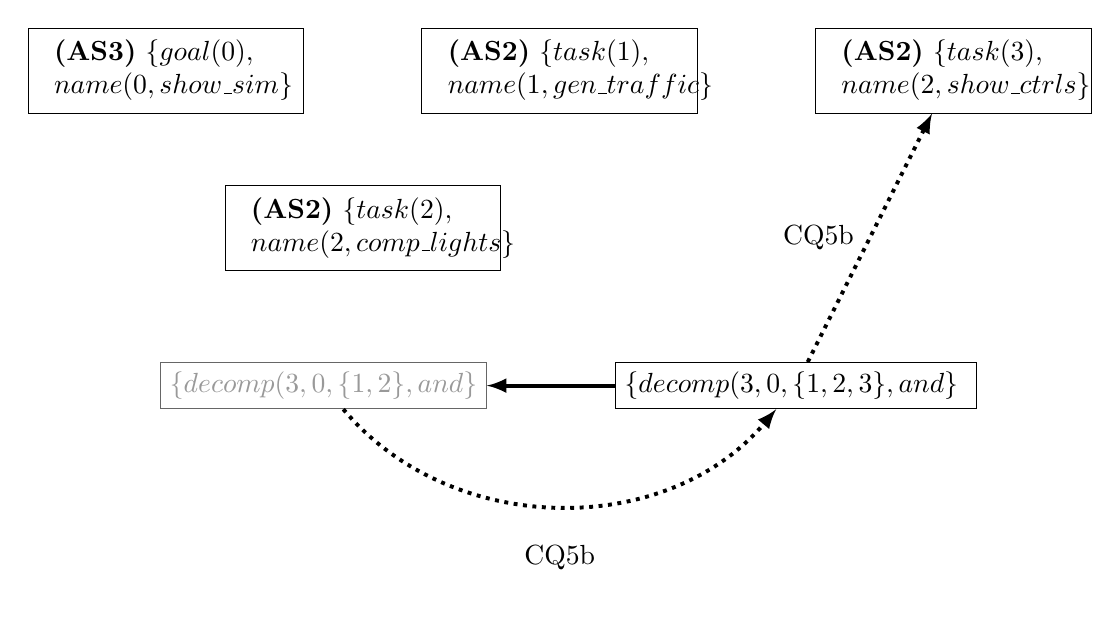
\begin{tikzpicture}
        \node (a0) [argNodeIN,minimum width=1.5cm] at (-5,0) {
        	\smallargtext{AS3}{$\{goal(0),$\\$name(0,show\_sim\}$}
        };
        \node (a1) [argNodeIN] at (0,0) {
        \smallargtext{AS2}{$\{task(1),$\\$name(1,gen\_traffic\}$}
        };
        \node (a2) [argNodeIN] at (5,0) {
        \smallargtext{AS2}{$\{task(3),$\\$name(2,show\_ctrls\}$}
        };
        \node (a2a) [argNodeIN] at (-2.5,-2) {
        \smallargtext{AS2}{$\{task(2),$\\$name(2,comp\_lights\}$}
        };
        \node (a3) [argNodeOUT] at (-3,-4) {$\{decomp(3,0,\{1,2\},and\}$
        };
        \node (a4) [argNodeIN] at (3,-4) {$\{decomp(3,0,\{1,2,3\},and\}$
        };
         
         \path
    (a4) edge [attackLink] (a3)
    (a3) edge [CQLink, bend right=50] node [below,draw=none] {CQ5b} (a4)
    (a4) edge [CQLink] node [left,draw=none] {CQ5b} (a2);
\end{tikzpicture}
\caption{Example of applying critical question CQ5b (Algorithm~\ref{alg:cq5b})}
\label{fig:examples:cq5b}
\end{figure*}

\noindent\textbf{Algorithms for critical questions CQ10a and CQ10b (REPLACE)}: These algorithms have a very similar structure as Algorithm~\ref{alg:cq5b} and have therefore been omitted.

\begin{algorithm}[h]
  \caption{Answering CQ13: ``Is the name of element $i$ clear?'' With: ``No, it should be $n$''}\label{alg:cq13}
  \begin{algorithmic}[1]
    \Procedure{CQ13}{$i, n$}
    \State $ArgsN \gets\{ A\in Args \mid name(i,x)\in A\}$
    \State $B\gets B'\backslash \{name(i,\_)\}$ with $B'\in ArgsN$
    \State $A \gets B \cup \{name(i,n)\}$
    \State $Args \gets Args \cup \{A\}$
    \For{$C$ in $ArgsN$}
      \State $Att\gets Att \cup \{(A,C)\}$
    \EndFor
    \EndProcedure
  \end{algorithmic}
\end{algorithm}

\noindent\textbf{Algorithms for critical question CQ13 (REPLACE):} \todo{F}{M}{deze moet aangepast worden nu de naam in het element staat} This algorithm is used to clarify/change the name of an element. It takes two parameters: the element identifier $i$ and the new name $n$. The idea behind the algorithm is that we construct a new argument for $n$, and to ensure that this argument attacks all previous arguments for giving a name to this element. Here we can use the following fact: Suppose $Args$ is a set of arguments, each containing an atom about the name for an element $i$, i.e. for all $A\in Args: name(i,_)\in Args$, then all arguments in $Args$ are the same except for the $name$ atoms, i.e. for all $A,B\in Args: A\backslash\{name(i,_)\} = B\backslash\{name(i,_)\}$. This means that if we would like to attack every argument of $Args$ with a new argument that replaces the $name$ atom, we can simply take any argument in $Args$, remove the previous $name$ atom, add the new one and attack all arguments in $Args$. This is exactly what the algorithm does.


On line 2, all arguments that have been put forward for this element and contain $name(i,x)$ are collected into the set $ArgsN$. On line 3, some arguments $B'\in ArgsN$ minus the $name$ statement is assigned to $B$ (note that it does not matter which one we pick), and on line 4 $B$ is joined with the new $name$ statement and stored in $A$, which is then added to the set of arguments $Args$. The for-loop on lines 6-8 ensures all previous arguments for names of the element are attacked by the new argument.

\begin{figure}[ht!]
\centering
        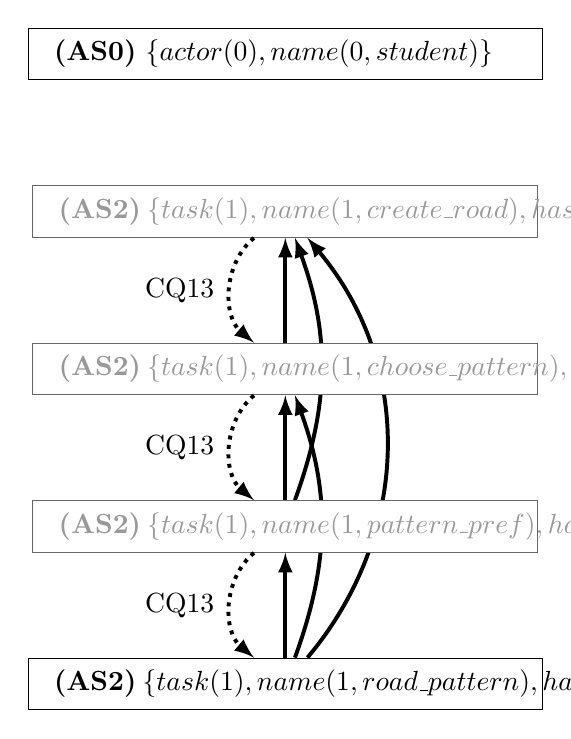
\begin{tikzpicture}[->]
        \node (a0a) [argNodeIN] at (-2,2) {
        	\longargtext{AS0}{$\{actor(0),name(0,student)\}$}
        };
        \node (a0) [argNodeOUT] at (-2,0) {
        	\longargtext{AS2}{$\{task(1),name(1,create\_road),has(0,1)\}$}
        };
        \node (a1) [argNodeOUT] at (-2,-2) {
        	\longargtext{AS2}{$\{task(1),name(1,choose\_pattern),has(0,1)\}$}
        };
        \node (a2) [argNodeOUT] at (-2,-4) {
        	\longargtext{AS2}{$\{task(1),name(1,pattern\_pref),has(0,1)\}$}
        };
        \node (a3) [argNodeIN] at (-2,-6) {
        	\longargtext{AS2}{$\{task(1),name(1,road\_pattern),has(0,1)\}$}
        };
\begin{pgfonlayer}{background}
         \path
    (a1) edge[attackLink] (a0)
    (a2) edge[attackLink] (a1)
    (a2) edge[attackLink, bend right=20] (a0)
    (a3) edge[attackLink] (a2)
    (a3) edge[attackLink, bend right=20] (a1)
    (a3) edge[attackLink, bend right=40] (a0);
\end{pgfonlayer}

	\path
	(a0) edge [CQLink, bend right=50] node [left,draw=none] {CQ13} (a1)
    (a1) edge [CQLink, bend right=50] node [left,draw=none] {CQ13} (a2)
    (a2) edge [CQLink, bend right=50] node [left,draw=none] {CQ13} (a3);
\end{tikzpicture}
\caption{Applying critical question CQ13 (Algorithm~\ref{alg:cq13}) to the example in Figure~\ref{fig:examples:clarification}.}
\label{fig:examples:clarification:formal}
\end{figure} 

An example of of Algorithm~\ref{alg:cq13} is shown in Figure~\ref{fig:examples:clarification:formal}. Let us consider the last application of CQ13 (bottom argument). Before this application, the following arguments have been put forward:
\begin{itemize}
\item $A_1$: $\{actor(0),name(0,student)\}$
\item $A_2$:$\{task(1),name(1,create\_road),has(0,1)\}$
\item $A_3$ $\{task(1),name(1,choose\_pattern),has(0,1)\}$
\item $A_4$:$\{task(1),name(1,pattern\_pref),has(0,1)\}$
\end{itemize}
The algorithm is now called as follows: $CQ13(1,road\_pattern)$, i.e., the new name of the element should be $road\_pattern$. Let us briefly run through the algorithm. After executing line 2 we obtain $ArgsN=\{A_2,A_3,A_4\}$, since only those arguments contain $name(1,\_)$. Next, on line 3, $B=\{task(1),has(0,1)\}$, i.e., $B$ is the general argument for the task without the $name$ statement. After line 4 we have $$A=\{task(1),has(0,1),name(1,road\_pattern),$$ which is added to $Args$ and attacks arguments $A_2,A_3$, and $A_4$. 

\noindent\textbf{Algorithms for critical questions CQ6b, CQ6c, CQ6d, CQ7b, and CQ9 (INTRO):} The introduction algorithms for the critical questions are all very similar to the INTRO algorithms for argument schemes (Algorithm~\ref{alg:as1}). They have therefore been omitted.

\begin{algorithm}[h]
  \caption{Generic counterargument to argument $A$}\label{alg:cq6b}
  \begin{algorithmic}[1]
    \Procedure{Attack}{$A$}
    \State $A_{new} = \{\}$
    \State $Args \gets Args \cup \{A_{new}\}$
    \State $Att \gets Att \cup \{(A_{new},A)\}$
    \EndProcedure
  \end{algorithmic}
\end{algorithm}

\noindent\textbf{Algorithm for $Att$ (Generic counter argument:} \todo{F}{M}{zoals je in Def 1 kunt zien heb ik generic arguments een id en een naam gegeven. Je moet ze namelijk kunnen aanvallen! (en de lege set kun je niet aanvallen want die is niet uniek te identificeren). algoritme moet dus aangepast worden}Applying a generic counter argument is very simple, and simply results on an attack on the original argument. We illustrate this by continuing our example from Figure~\ref{fig:examples:relevant-actor2:formal} (Algorithm~\ref{alg:as0}). The example is shown in Figure~\ref{fig:examples:relevant-actor2:formal}, where we see that a generic counter argument simply attacks the argument to disable the actor.

\begin{figure}[ht!]
\centering
        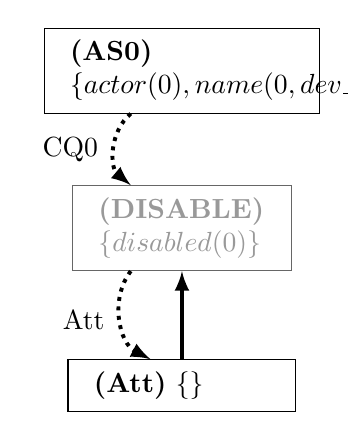
\begin{tikzpicture}
        \node (a0) [argNodeIN] at (-3.7,0) {
        	\smallargtext{AS0}{$\{actor(0),name(0,dev\_team\}$}
        } ;
        \node (a1) [argNodeOUT] at (-3.7,-2){
        	\argtext{DISABLE}{$\{disabled(0)\}$}
        };
        \node (a2) [argNodeIN] at (-3.7,-4){
        	\argtext{Att}{$\{\}$}
        };
         \path
    (a0) edge [CQLink, bend right=50] node [left,draw=none] {CQ0} (a1)
    (a1) edge [CQLink, bend right=50] node [left,draw=none] {Att} (a2)
    (a2) edge [attackLink] (a1);
\end{tikzpicture}
\caption{Formalization of the arguments in Figure~\ref{fig:examples:relevant-actor2}.}
\label{fig:examples:relevant-actor2:formal}
\end{figure}

\subsection{Constructing GRL models}
\label{sect:rationalGRL-GRL}
\todo{F}{F,M}{Dit is snel getypt, moet nog checken of het klopt.}

\begin{definition}[RationalGRL model] A RationalGRL model $\mathcal{R}$ is an argumentation framework $AF=(Args,Att)$ where all arguments in $Args$ and attacks in $Att$ are based on algorithm X-XX.  
\end{definition}

\begin{definition}[GRL model] A GRL model $\mathcal{M}$ based on a RationalGRL model $\mathcal{R}$ is the preferred extension of $\mathcal{R}$.  
\end{definition}

Constructing GRL models from the arguments is extremely simple: We simply compute the extensions of the argumentation frameworks, and collect all atomic sentences in the accepted arguments. This forms out GRL model. Let us briefly do so for the examples of the previous subsection:
\begin{itemize}
\item
Figure~\ref{fig:examples:relevant-actor:formal}: Since there are no attacks between the arguments, all atomic sentences are accepted. This results in the following specification: 
\begin{quote}
\begin{verbatim}
actor(0).
name(0,dev_team).
disabled(0).
\end{verbatim}
\end{quote}
This again corresponds to the GRL model on the right-hand side of Figure~\ref{fig:examples:relevant-actor}.
\item
Figure~\ref{fig:examples:cq5b}: There is one rejected argument and five accepted ones. The resulting specification is:
\begin{quote}
\begin{verbatim}
goal(0). name(0,show_simulation).
task(1). name(1,generate_traffic).
task(2). name(2,compute_lights).
task(3). name(3,show_controls).
decomp(3,0,{1,2,3},and).
\end{verbatim}
\end{quote}
\item Figure~\ref{fig:examples:clarification:formal}: There are only two accepted arguments. The resulting specification is:
\begin{quote}
\begin{verbatim}
actor(0). name(0, student).
task(1).  name(1,road_pattern).
has(0,1).
\end{verbatim}
\end{quote}
This corresponds to the right-hand GRL model of Figure~\ref{fig:examples:clarification}.
\item Figure~\ref{fig:examples:relevant-actor2:formal}. There are two accepted arguments, but the \emph{generic counterargument} does not contain any formulas. Therefore the resulting specification is:
\begin{quote}
\begin{verbatim}
actor(0).
name(0,dev_team).
\end{verbatim}
\end{quote}
This corresponds to the right-hand GRL model of Figure~\ref{fig:examples:relevant-actor2}.
\end{itemize}
\section{The RationalGRL Tool}
\label{sect:implementation}

\todo{Marc}{Marc}{Currently this section comes from my thesis where I present the tool as future work. Here we should explain it}

GRL has a well-documented and well-maintained tool called jUCMNav~\cite{jUCMNav}. This tool is an extension to Eclipse. Although it is a rich tool with many features, we also believe it is not very easy to set it up. This seriously harms the exposure of the language, as well as the ability for practitioners to use it. We have started to implement a simple version of GRL as an online tool in Javascript. This makes it usable from the browser, without requiring the installation of any tool. The tool can be used from the following address:

\begin{quote}
\url{http://marcvanzee.nl/RationalGRL/editor}
\end{quote}

A screenshot of the tool is shown in Figure~\ref{fig:goalmodeling:tool}. As shown, there are two tabs in the tool, one for ``Argument'' and one for ``GRL''. The argument part has not been implemented yet, and the GRL part only partly, but the idea behind the tool should be clear. Users are able to work on argumentation and on goal modeling in parallel, where the argumentation consists of forming arguments and counterarguments by instantiating argument schemes and answering critical questions. 

\begin{figure*}[h!]
\centering
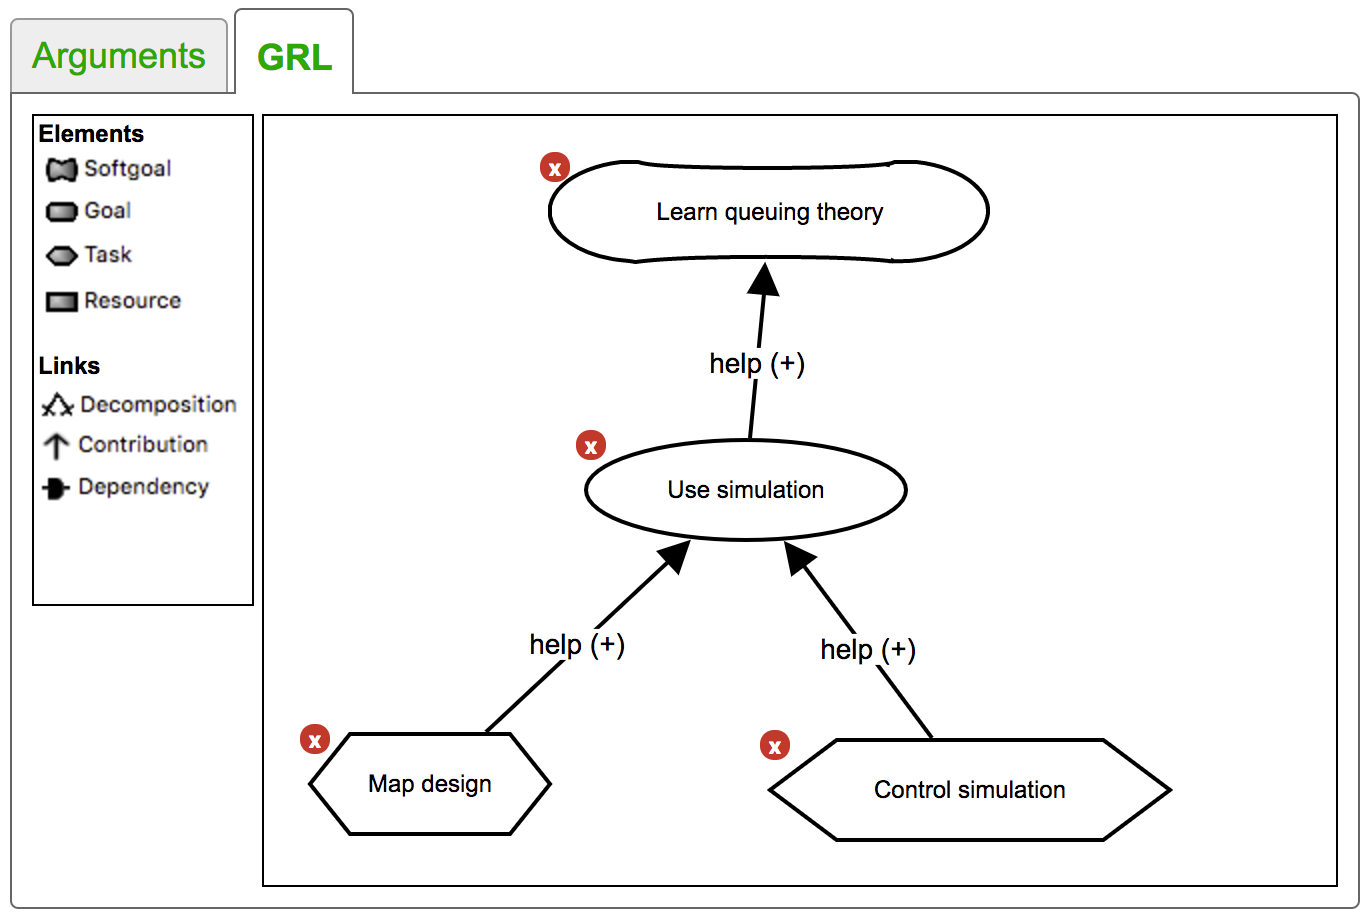
\includegraphics[scale=0.5]{img/tool_screen}
\caption{Screenshot of the prototype tool}
\label{fig:goalmodeling:tool}
\end{figure*}

An important aspect of the tool is that users can switch freely between these two ways of modeling the problem. One can model the entire problem in GRL, or one can do everything using argumentation. However, we believe the most powerful way to do so is to switch back and forth. For instance, one can create a simple goal model in GRL, and then turn to the argumentation part, which the users can look at the various critical questions for the elements, which may trigger discussions. These discussions results in new arguments for and against the elements in the goal model. Once this process is completed, one may switch to the goal model again, and so on. We believe that in this way, there is a close and natural coupling between modeling the goals of an organization as well as rationalizing them with arguments.
\section{Discussion}
\label{sect:goalmodeling:discussion}

\subsection{Related work}
\label{sect:goalmodeling:relatedwork}

The need for justifications of modeling choices plays an important role in different requirements engineering methods using goal models. High-level goals are often understood as reasons for representing lower-level goals (in other words, the need for low-level goals is justified by having high-level goals) and other elements in a goal model such as tasks and resources. Various refinements and decomposition techniques,  often used in requirements engineer (See~\cite{EP-2001-Lamsweerde-GORE} for an overview), can be seen as incorporating argumentation and justification, in that sub-goals could be understood as arguments supporting parent goals. In that case, a refinement alternative is justified if there are no conflicts between sub-goals (i.e., it is consistent), as few obstacles as possible sub-goals harm sub-goal achievement, there are no superfluous sub-goals (the refinement is minimal), and the achievement of sub-goals can be verified to lead to achieving the parent goal (if refinement is formal~\cite{Darimont:1996:FRP:239098.239131}). This interpretation is one of the founding ideas of goal modeling. However, while this interpretation may seem satisfactory, argumentation and justification processes differ from and are complementary to refinement in several respects, such as limited possibilities for rationalization and lack of semantics (see Jureta~\cite{Jureta:RE2008} for more details).

There are several contributions that relate argumentation-based techniques with goal modeling. The contribution most closely related to ours is the work by Jureta \emph{et al.}~\cite{Jureta:RE2008}. Jureta \emph{et al.} propose ``Goal Argumentation Method (GAM)'' to guide argumentation and justification of modeling choices during the construction of goal models. One of the elements of GAM is the translation of formal argument models to goal models (similar to ours). In this sense, our RationalGRL framework can be seen as an instantiation and implementation of  part of the GAM. The main difference between our approach and GAM is that we integrate arguments and goal models using argument schemes, and that we develop these argument schemes by analyzing transcripts. GAM instead uses structured argumentation. 

The RationalGRL framework is also closely related to frameworks that aim to provide a design rationale (DR)~\cite{shum2006hypermedia}, an explicit documentation of the reasons behind decisions made when designing a system or artefact. DR looks at issues, options and arguments for and against the various options in the design of, for example, a software system, and provides direct tool support for building and analyzing DR graphs. One of the main improvements of RationalGRL over DR approaches is that RationalGRL incorporates the formal semantics for both argument acceptability and goal satisfiability, which allow for a partly automated evaluation of goals and the rationales for these goals. 

Arguments and requirements engineering approaches have been combined by, among others, Haley \emph{et al.}~\cite{haley2005arguing}, who use structured arguments to capture and validate the rationales for security requirements. However, they do not use goal models, and thus, there is no explicit trace from arguments to goals and tasks. Furthermore, like~\cite{Jureta:RE2008}, the argumentative part of their work does not include formal semantics for determining the acceptability of arguments, and the proposed frameworks are not actually implemented. Murukannaiah \emph{et al.}~\cite{murukannaiah2015resolving} propose Arg-ACH, an approach to capture inconsistencies between stakeholders' beliefs and goals, and resolve goal conflicts using argumentation techniques.

\subsection{Open issues}
\label{sect:goalmodeling:openissues}

We see a large number of open issues that we hope will be explored in future research. We discuss five promising directions here.

\subsubsection*{Architecture principles} 
One aspect of enterprise architecture that we did not touch upon in this article are \emph{(enterprise) architecture principles}. Architecture principles are general rules and guidelines, intended to be enduring and seldom amended, that inform and support the way in which an organization sets about fulfilling its mission~\cite{Lankhorst2005,OptLand2007a,OG2009}. They reflect a level of consensus among the various elements of the enterprise, and form the basis for making future IT decisions. Two characteristics of architecture principles are:
\begin{itemize}
\item There are usually a small number of principles (around 10) for an entire organization. These principles are developed by enterprise architecture, through discussions with stakeholders or the executive board. Such a small list is intended to be understood \emph{throughout the entire organization}. All employees should keep these principles in the back of their hard when making a decision.
\item Principles are meant to guide decision making, and if someone decides to deviate from them, he or she should have a good reason for this and explain why this is the case. As such, they play a normative role in the organization.
\end{itemize}

Looking at these two characteristics, we see that argumentation, or justification, plays an important role in both forming the principles and adhering to them:
\begin{itemize}
\item Architecture principles are \emph{formed} based on underlying arguments, which can be the goals and values of the organization, preferences of stakeholders, environmental constraints, etc.
\item If architecture principles are \emph{violated}, this violation has to be explained by underlying arguments, which can be project-specific details or lead to a change in the principle.
\end{itemize}

In a previous paper, we~\cite{marosin-etal:caise2016} propose an extension to GRL based on enterprise architecture principles. We present a set of requirements for improving the clarity of definitions and develop a framework to formalize architecture principles in GRL. We introduce an extension of the language with the required constructs and establish modeling rules and constraints. This allows one to automatically reason about the soundness, completeness and consistency of a set of architecture principles. Moreover, principles can be traced back to high-level goals.

It would be very interesting future work to combine the architecture principles extension with the argumentation extension. This would lead to a framework in which principles cannot only be traced back to goals, but also to underlying arguments by the stakeholders.

\subsubsection*{Extensions for argumentation}

The amount of argumentation theory we used in this article has been rather small. Our intention was to create a bridge between the formal theories in argumentation and the rather practical tools in requirements engineering. Now that the initial framework has been developed, is it worth exploring what tools and variations formal argumentation has to offer in more detail.

For instance, until now we have assumed that every argument put forward by a critical questions always defeats the argument it questions, but this is a rather strong assumption.  In some cases, it is more difficult to determine whether or not an argument is defeated. Take, for example, the argumentation framework in Figure~\ref{fig:goalmodeling:futureargs} with just A1 and A2. These two arguments attack each other, they are alternatives and without any explicit preference, and it is impossible to choose between the two. It is, however, possible to include explicit preferences between arguments when determining argument acceptability \cite{amgoud2002reasoning}. If we say that we prefer the action  \texttt{Create new cars} (A2) over the action  \texttt{Keep same cars} (A1), we remove the attack from A1 to A2. This makes A2 the only undefeated argument, whereas A1 is now defeated. It is also possible to give explicit arguments for preferences~\cite{modgil2009}. These arguments are then essentially attacks on attacks. For example, say we prefer A3 over A1 because `it is important to have realistic traffic flows' (A4). This can be rendered as a separate argument that attacks the attack from A1 to A3, removing this attack and making $\{$A3, A4$\}$ the undefeated set of arguments.

Allowing undefeated attacks also make the question of which semantics to choose more interested. In our current (a-cyclic) setting, all semantics coincide, and we always have the same set of accepted arguments. However, once we allow for cycles, we may choose accepted arguments based on semantics which, for instance, try to accept/reject as many arguments as possible (preferred semantics), or just do not make any choice once there are multiple choices (grounded). Another interesting element of having cycles is that one can have multiple extensions. This corresponds to various \emph{positions} are possible, representing various sets of possibly accepted arguments. Such sets can then be shown to the user, who can then argue about which one they deem most appropriate.


\begin{figure}[ht]
\centering
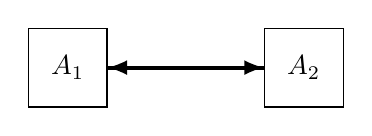
\begin{tikzpicture}
        \node[minimum size=1cm] (a1) [argNodeIN] at (0,0) {$A_1$};
        \node[minimum size=1cm] (a2) [argNodeIN] at (3,0) {$A_2$};
        
         \path
    (a2) edge [attackLink] (a1)
    (a1) edge [attackLink] (a2);
\end{tikzpicture}
\caption{Preferences between arguments}
\label{fig:goalmodeling:futureargs}
\end{figure}  

Finally, in this article we have only explored one single argument scheme, but there are many other around. In his famous book ``Argumentation schemes'', Walton describes a total of 96 schemes. Murukannaiah \emph{et al.}~\cite{murukannaiah2015} already explain how some of these schemes may be use for resolving goal conflicts, and it is worth studying what this would look like in our framework as well.

\subsubsection*{Empirical study}

Although we develop our argument schemes and critical questions with some empirical data, we did not yet validate the outcome. This is an important part, because it will allow us to understand whether adding arguments to goal modeling is actually useful. We have developed an experimental setup for our experiment, which we intend to do during courses at various universities. However, we cannot carry out this experiment until the tool is finished.

\subsubsection*{Formal framework}

The formal framework we present in this article is very simple, and does not provide a lot of detail. We believe it would be interesting to develop a more robust characterization of a GRL model using logical formulas. Right now, we have no way to verify whether the goal models we obtain through out algorithms are actually valid GRL models. This is because we allow any set of atoms to be a GRL model, which is clearly very permissive and incorrect. Once we develop a number of such constraints, we can ensure (and even proof) our algorithms do not generate invalid GRL models. 

For instance, suppose we assert that an \emph{intentional element} is a goal, softgoal, task, or resource: \begin{align*}
(softgoal(i)\vee goal(i)\vee task(i)\\
\vee resource(i)\rightarrow IE(i).
\end{align*}
We can then formalize an intuition such as: ``Only intentional elements can be used in contribution relations'' as follows
\begin{align*}
contrib(k,i,j,ctype)\rightarrow \\
(IE(i)\wedge IE(j)\wedge IE(j).
\end{align*}

Interestingly, such constraints are very comparable to \emph{logic programming} rules. We therefore see it as interesting future research to explore this further, specifically in the following two ways:
\begin{itemize}
\item Develop a set of constraints on sets of atoms of our language, which correctly describe a GRL model. Show formally that using our algorithms, each extension of the resulting argumentation framework corresponds to a valid GRL model, i.e., a GRL model that does not violate any of the constraints.
\item Implement the constraints as a logic program, and use a logic programming language to compute the resulting GRL model.
\end{itemize}


\subsection{Conclusion}

In this article, we develop the RationalGRL framework to trace back elements of GRL models to arguments using in discussions between stakeholders. The contributions of this article have become increasingly more formal. First, we analyze transcripts of meetings about the development of an information system. We count occurrences of argument schemes and critical questions, and categorize them by the effect of instantiating them. Then, we create a visual notation to link arguments and questions to elements of a goal model. If an argument for an element of a goal model is rejected, then the corresponding element is disabled. Similarly, if the argument is accepted, then the corresponding element is enabled. Finally, we formalize the argument schemes and critical questions in a logical framework. We propose a formal language to describe a GRL model, and we develop various algorithms for applying our argument schemes and critical questions. 

Our framework is one of the first attempts that try to combine the formal theory of argumentation with the practical frameworks of goal modeling. History has shown that it is remarkably difficult to combine formal results with practice. By taking argument schemes as a starting point, we believe we have chosen the right level of formality, but as the open issues section shows, much work is left to be done. 

\bibliographystyle{abbrv}
\bibliography{references}

\newpage

\onecolumn
\appendix

\section{UCI Design Workshop Prompt}
\label{sect:designprompt}

\subsection*{Design Prompt: Traffic Signal Simulator}

\subsubsection*{Problem Description}

For the next two hours, you will be tasked with designing a traffic flow simulation program. Your client for this project is Professor E, who teaches civil engineering at UCI. One of the courses she teaches has a section on traffic signal timing, and according to her, this is a particularly challenging subject for her students. In short, traffic signal timing involves determining the amount of time that each of an inter- section's traffic lights spend being green, yellow, and red, in order to allow cars in to flow through the intersection from each direction in a fluid manner. In the ideal case, the amount of time that people spend waiting is minimized by the chosen settings for a given intersection's traffic lights. This can be a very subtle matter: changing the timing at a single intersection by a couple of seconds can have far- reaching effects on the traffic in the surrounding areas. There is a great deal of theory on this subject, but Professor E. has found that her students find the topic quite abstract. She wants to provide them with some software that they can use to ``play'' with different traffic signal timing schemes, in different scenarios. She anticipates that this will allow her students to learn from practice, by seeing first-hand some of the patterns that govern the subject.

\subsubsection*{Requirements}
The following broad requirements should be followed when designing this system:
\begin{enumerate}
\item
Students must be able to create a visual map of an area, laying out roads in a pattern of their choosing. The resulting map need not be complex, but should allow for roads of varying length to be placed, and different arrangements of intersections to be created. Your approach should readily accommodate at least six intersections, if not more.
\item
Students must be able to describe the behavior of the traffic lights at each of the intersections. It is up to you to determine what the exact interaction will be, but a variety of sequences and timing schemes should be allowed. Your approach should also be able to accommodate left-hand turns protected by left-hand green arrow lights. In addition:
\begin{enumerate}
\item
Combinations of individual signals that would result in crashes should not be allowed.
\item
Every intersection on the map must have traffic lights (there are not any stop signs, over- passes, or other variations). All intersections will be 4-way: there are no ``T'' intersections, nor one-way roads.
\item
Students must be able to design each intersection with or without the option to have sensors that detect whether any cars are present in a given lane. The intersection's lights' behavior should be able to change based on the input from these sensors, though the exact behavior of this feature is up to you.
\end{enumerate}
\item
Based on the map created, and the intersection timing schemes, the students must be able to simulate traffic flows on the map. The traffic levels should be conveyed visually to the user in a real-time manner, as they emerge in the simulation. The current state of the intersections' traffic lights should also be depicted visually, and updated when they change. It is up to you how to present this information to the students using your program. For example, you may choose to depict individual cars, or to use a more abstract representation.
\item
Students should be able to change the traffic density that enters the map on a given road. For ex- ample, it should be possible to create a busy road, or a seldom used one, and any variation in between. How exactly this is declared by the user and depicted by the system is up to you. Broadly, the tool should be easy to use, and should encourage students to explore multiple alternative approaches. Stu- dents should be able to observe any problems with their map's timing scheme, alter it, and see the results of their changes on the traffic patterns. This program is not meant to be an exact, scientific simulation, but aims to simply illustrate the basic effect that traffic signal timing has on traffic. If you wish, you may assume that you will be able to reuse an existing software package that provides relevant mathematical functionality such as statistical distributions, random number generators, and queuing theory.
\end{enumerate}

You may add additional features and details to the simulation, if you think that they would support these goals.

Your design will primarily be evaluated based on its elegance and clarity – both in its overall solution and envisioned implementation structure.

\subsubsection*{Desired Outcomes}

Your work on this design should focus on two main issues:

\begin{enumerate}
\item
You must design the interaction that the students will have with the system. You should design the basic appearance of the program, as well as the means by which the user creates a map, sets traffic timing schemes, and views traffic simulations.
\item
You must design the basic structure of the code that will be used to implement this system. You should focus on the important design decisions that form the foundation of the implementation, and work those out to the depth you believe is needed.
\end{enumerate}

The result of this session should be: \emph{the ability to present your design to a team of software developers who will be tasked with actually implementing it.} The level of competency you can expect is that of students who just completed a basic computer science or software engineering undergraduate degree. You do not need to create a complete, final diagram to be handed off to an implementation team. But you should have an understanding that is sufficient to explain how to implement the system to competent developers, without requiring them to make many high-level design decisions on their own.

To simulate this hand-off, you will be asked to briefly explain the above two aspects of your design after the design session is over.

\subsubsection*{Timeline}
\begin{itemize}
\item 1 hour and 50 minutes: Design session
\item 10 minutes: Break / collect thoughts
\item 10 minutes: Explanation of your design 
\item 10 minutes: Exit questionnaire
\end{itemize}
\newpage
\section{Transcripts excerpts}
\label{sect:transcripts:excerpts}

\begin{table}[!htbp]
\centering
\begin{tabular}{|p{20mm}|p{70mm}|p{60mm}|}
\hline
Respondent & Text & Annotation\\
\hline
0:10:55.2 (P1) & Maybe developers &\textbf{[4 actor (AS0)]} Development team\\
\hline
0:11:00.8 (P2) & Development team, I don't know. Because that's- in this context it looks like she's gonna make the software & \textbf{[5 critical question CQ0 for 4]} Is actor "development team" relevant?\newline
\textbf{[6 answer to 5]} No, it looks like the professor will develop the software.\\
\hline
\end{tabular}
\caption{AS0: Actor, CQ0: Relevant actor? (transcript $t_3$)}
\label{table:transcript:as0-cq0}

\begin{tabular}{|p{20mm}|p{70mm}|p{60mm}|}
\hline
Respondent & Text & Annotation\\
\hline
0:19:08.6 (P3) & Should have a link with an outsource program for the statistical distribution [inaudible] & \textbf{[21 resource (AS1)]} Actor System has resource ``Statistics library''\\
\hline
0:35:27.4 (P3) & Maybe before traffic simulation view you can- the outsource package that makes the map	& \textbf{[38 contribution (AS8)]} Resource ``Statistics library'' contributes to task ``Display traffic simulation''\\
\hline
\end{tabular}
\caption{AS1: Resource, AS8: Resource contributes to task (transcript $t_3$)}
\label{table:transcript:as1-as8}

\begin{tabular}{|p{20mm}|p{70mm}|p{60mm}|}
\hline
Respondent & Text & Annotation\\
\hline
0:15:11.2 (P1) & And then, we have a set of actions. Save map, open map, add and remove intersection, roads & \multirow{2}{60mm}{\textbf{[20 task (AS2)]} Student has tasks ``save map'', ``open map'', ``add intersection'', ``add road'', ``add traffic light'', ``remove intersection''}\\
\cline{1-2}
0:15:34.7 (P2) & Yeah, road. Intersection, add traffic lights	&\\
\hline
0:15:42.3 (P1) & Well, all intersection should have traffic lights so it's & \textbf{[21 critical question CQ*1 for 20]} Is the task ``Add traffic light'' useful/redundant? \newline
\textbf{[22 answer to 22]} Not useful, because according to the specification all intersections have traffic lights.\\
\hline
0:15:52.3 (P1) & (..) And on the technical side it's gonna be a real pain to remove one intersection you're gonna have to remove a lot more because there are only four-ways allowed and if you remove one intersection then-& \textbf{[23 critical question CQ2 for 20]} Is the task ``Remove intersection'' possible?\newline
\textbf{[24 answer to 22]} It is going to be very difficult to implement.\\
\hline
\end{tabular}
\caption{AS2: Task, CQ*1: Redundant element, CQ2: impossible task (transcript $t_1$)}
\label{table:transcript:as2-cq_star_1-cq2}

\begin{tabular}{|p{20mm}|p{70mm}|p{60mm}|}
\hline
Respondent & Text & Annotation\\
\hline
0:23:20.4 (P1) & So, sets, yeah, car influx & \textbf{[32 task (AS2)]} Student has task ``car influx''\\
\hline
0:23:41.2 (P2) & (..) If you can only control the set amount of influx from any side of this sort of random distribution, I think that is going to be less interesting than when you can say something like, this road is frequently traveled. (...) So setting it per road, I think is something we want & \textbf{[33 critical question CQ*2 on 36]} Is the task description specific/clear enough? \newline
\textbf{[34 answer to 37]} No, it is not clear where the influx is changing. Change to ``control car influx per road''\\
\hline
\end{tabular}
\caption{AS2: Task, CQ*2: Specify/clarify element (transcript $t_1$)}
\label{table:transcript:as2-cq_star_2}

\begin{tabular}{|p{20mm}|p{50mm}|p{80mm}|}
\hline
Respondent & Text & Annotation\\
\hline
0:14:31.2 (P1) & Let's see- she uses the system in her course to explain her lectures about traffic problem thing & \textbf{[11 softgoal (AS4)]} ``Explain lectures traffic theory'' (Professor)\newline
\textbf{[12 goal (AS5)]} ``Use traffic light system'' (Professor)\newline
\textbf{[13 contribution (AS7)]} ``use traffic light system'' contributes to ``explain lectures traffic theory''\\
\hline
\end{tabular}
\caption{AS4: softgoal, AS5: goal, AS7: contribution (transcript $t_3$)}
\label{table:transcript:as4-as5-as7}

\begin{tabular}{|p{20mm}|p{90mm}|p{40mm}|}
\hline
Respondent & Text & Annotation\\
\hline
0:00:10.2\newline PERSON 1 & 	So, yeah [pause] I would start with something about the context. That we have to determine who the users of the system are gonna be, stakeholders. & \textbf{[1 topic]} What are the actors?\\
\hline
\end{tabular}
\caption{AS*: Topic introduction (transcript $t_1$)}
\label{table:transcript:as-star}
\end{table}

\begin{table}[!htbp]
\centering
\begin{tabular}{|p{20mm}|p{70mm}|p{60mm}|}
\hline
Respondent & Text & Annotation\\
\hline
0:29:59.5 (P3) & (...) a variety of sequences and timing schemes should be allowed.  (...) we would have traffic light behavior gives you, I guess two options then. & \multirow{4}{60mm}{\textbf{[42 task (AS2)]} Student has task ``set sequence scheme''\newline
\textbf{[43 task (AS2)]} Student has task ``set timing scheme'' \newline
\textbf{[44 decomposition (AS10)] }Task ``set traffic light behavior'' XOR-decomposes into ``set sequence scheme'' and ''set timing scheme''}\\
\cline{1-2}
0:30:23.6 (P1) & Sequences and timing schemes &\\
\cline{1-2}
0:30:25.0 (P3) & Sequences and timing schemes. So you can either go for, yeah, sequences-&\\
\cline{1-2}
0:30:30.9 (P1) & Or timing schemes&\\
\hline	
\end{tabular}
\caption{AS2: Task, AS10: Task decomposition (transcript $t_2$)}
\label{table:transcript:as2-as10}

\begin{tabular}{|p{20mm}|p{70mm}|p{60mm}|}
\hline
Respondent & Text & Annotation\\
\hline
0:30:10.3 (P1) & 	Yeah. But this is- is this an OR or an AND? & \multirow{3}{60mm}{\textbf{[26 critical question CQ*0 for 20]} Is the OR-decomposition of ``simulate'' correct?\newline
\textbf{[27 answer to 26]} No, it should be an AND because the system can do both.}\\
\cline{1-2}
0:30:14.3 (P3) &I think it's an OR&\\
\cline{1-2}
0:30:15.4 (P1) & for the data, it's an OR (...) And for the system it's an AND. (...) Static manner or dynamic. But the system can do both&\\
\hline	
\end{tabular}
\caption{CQ11b: Incorrect decomposition (transcript $t_3$)}
\label{table:transcript:cq11b}

\begin{tabular}{|p{20mm}|p{100mm}|p{30mm}|}
\hline
Respondent & Text & Annotation\\
\hline
0:06:29.3 (P2) & So, is that a trade-off. I think so. &\multirow{2}{30mm}{\textbf{[10 negative contribution (AS11)]}  task ``generate cars randomly'' contributes negatively to softgoal ``dynamic simulation''}\\	
\cline{1-2}
0:06:36.0 (P1) & Yeah, performance versus, I don't know, functionality. Like, what you say, cars come out at the end of the map side [are generated randomly] is performance wise and, I don't know, easier to make but it is less functional. Because you can't see traffic flows that easy because, well there's fixed amount of cars so there's not really gonna be jams [the simulation is less dynamic]. Is there around Utrecht always the same amount of cars? &\\
\hline	
\end{tabular}
\caption{AS11: Negative decomposition (transcript $t_1$)}
\label{table:transcript:as11}

\begin{tabular}{|p{20mm}|p{80mm}|p{50mm}|}
\hline
Respondent & Text & Annotation\\
\hline
0:49:05.3 (P3)&So, density, speed and, is there anything else.&\multirow{3}{50mm}{\textbf{[68 critical question for 63c]} Does ``set road characteristics'' decompose into any other tasks?\newline
\textbf{[69 answer to 68]} Yes, type of cars.}\\
\cline{1-2}
0:49:20.1 (P1) & Maybe type of cars&\\	
\cline{1-2}
0:49:22.0 (P3) & Type of cars, because you could have trucks, you could have personal cars. That would be good because-&\\
\hline	
\end{tabular}
\caption{CQ: Does a task decompose into other tasks? (transcript $t_2$)}
\label{table:transcript:cq:task_decomp}

\begin{tabular}{|p{20mm}|p{60mm}|p{70mm}|}
\hline
Respondent & Text & Annotation\\
\hline

0:10:55.2 (P1) & Maybe developers or & \textbf{[4 actor (AS0)]} Development team\\
\hline
0:11:00.8 (P2)&Development team, I don't know. Because that's- in this context it looks like she's gonna make the software&\textbf{[5 critical question CQ0 for 4]} Is actor ``development team'' relevant?\newline
\textbf{[6 answer to 5]} No, it looks like the professor will develop the software.\\
\hline
..&..&..\\
\hline
0:18:13.4 (P2) & I think we can still do developers here. To the system & \multirow{2}{70mm}{\textbf{[16 counter argument for 6]} According to the specification the professor doesn't actually develop the software.}\\
\cline{1-2}
0:18:22.9 (P1)&Yeah, when the system gets stuck they also have to be [inaudible] ok. So development team&\\	
\hline	
\end{tabular}
\caption{AS0: Task, CQ0: Relevant task? CQ: Generic counterargument (transcript $t_2$)}
\label{table:transcript:as0-cq0-cq_counterarg}

\end{table}

\newpage
\section{Tool screenshots}
\label{sect:tool-screenshots}

\begin{figure}[ht]
\centering
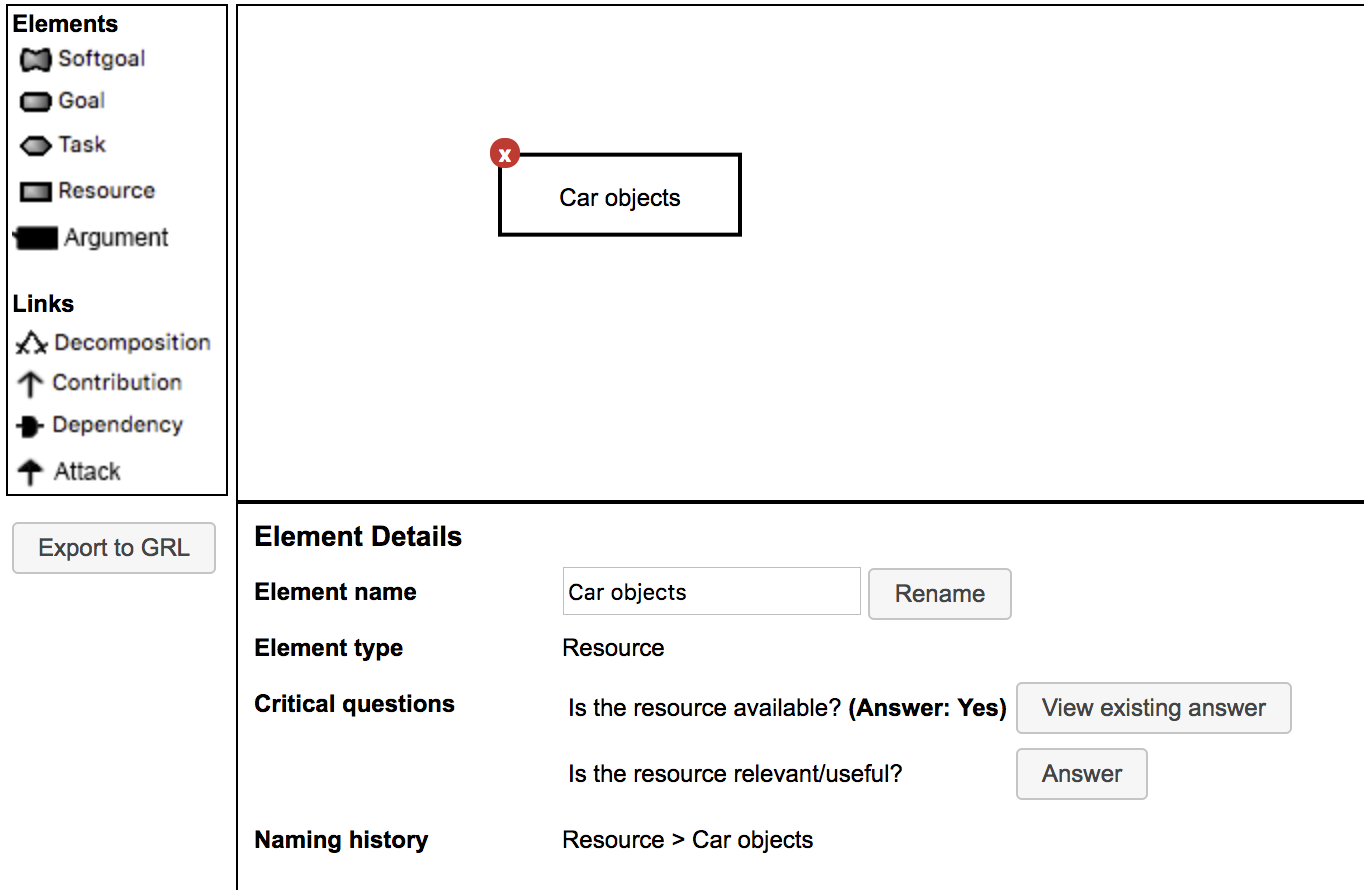
\includegraphics[scale=0.6]{img/tool-overview}
\caption{Overview of the RationalGRL tool}
\label{fig:tool:overview}
\end{figure}

\begin{figure}[ht]
\centering
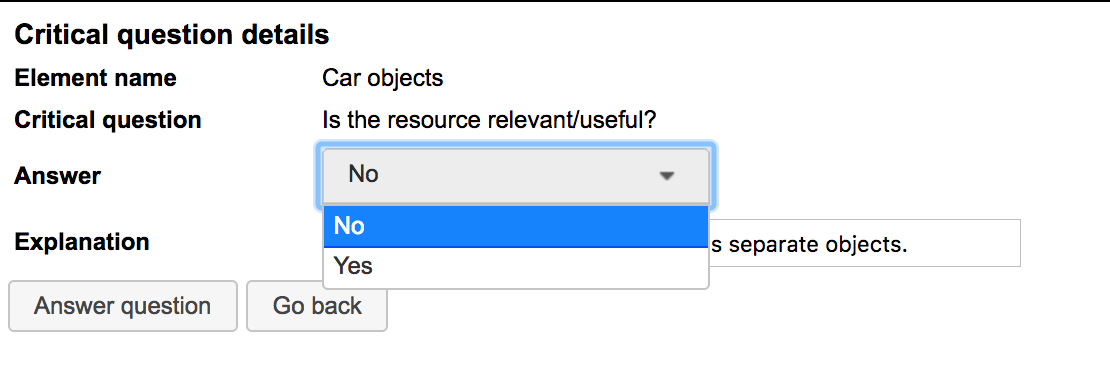
\includegraphics[scale=0.6]{img/tool-cqdetails}
\caption{Critical question details pane for ``Is the resource relevant/useful?''}
\label{fig:tool:cqdetails}
\end{figure}

\newpage

\begin{figure}[ht]
\centering
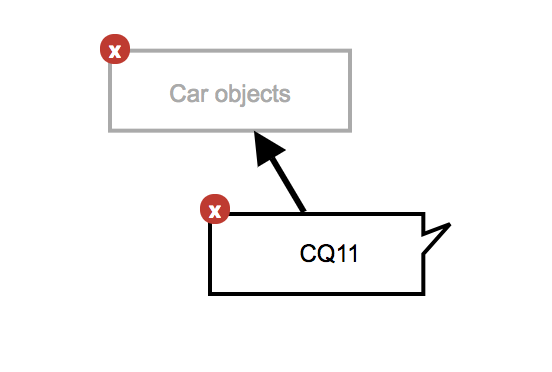
\includegraphics[scale=0.6]{img/tool-cqeffect}
\caption{Effect of answering CQ11: ``Is the resource reelevant/useful?'' with ``No''}
\label{fig:tool:cqeffect}
\end{figure}

\begin{figure}[ht]
\centering
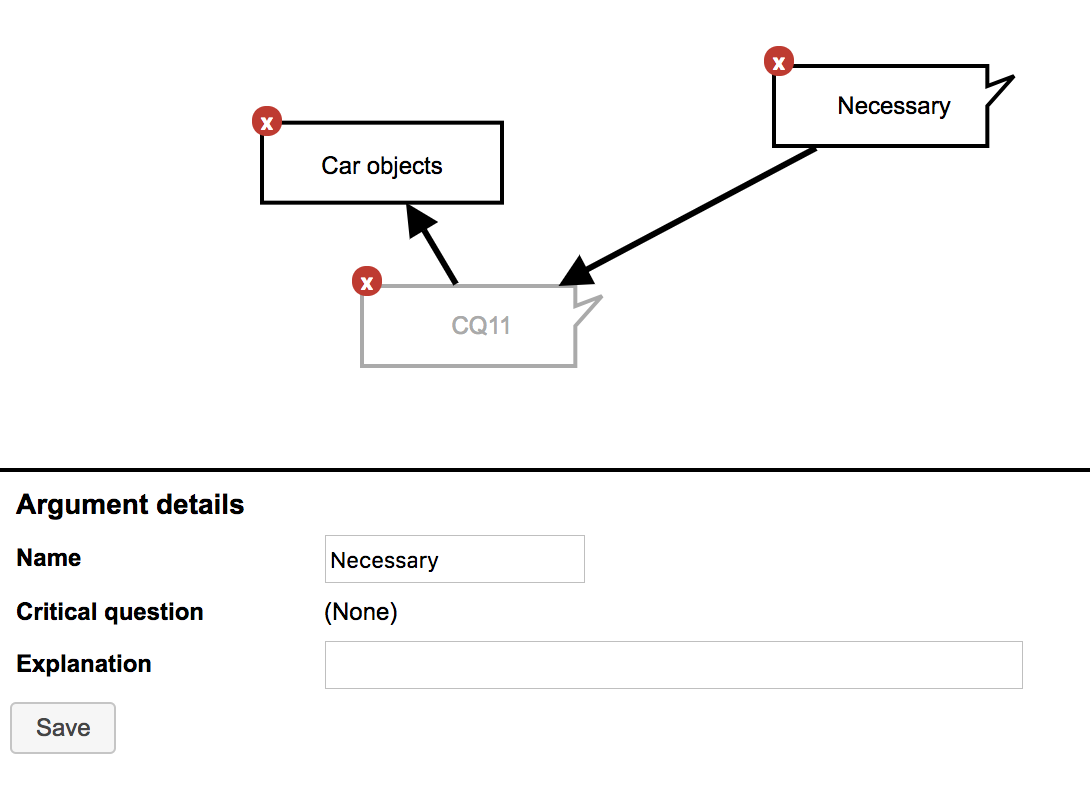
\includegraphics[scale=0.5]{img/tool-argument}
\caption{Argument details pane for generic argument ``Necessary''}
\label{fig:tool:argument}
\end{figure}

\begin{figure}[ht]
\centering
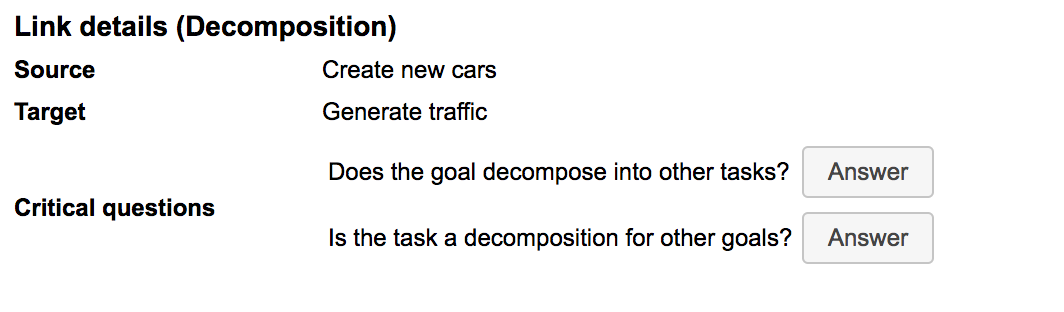
\includegraphics[scale=0.5]{img/tool-linkdetails}
\caption{Link details pane for decomposition link}
\label{fig:tool:cqdetails}
\end{figure}

\newpage

\begin{figure}[ht]
\centering
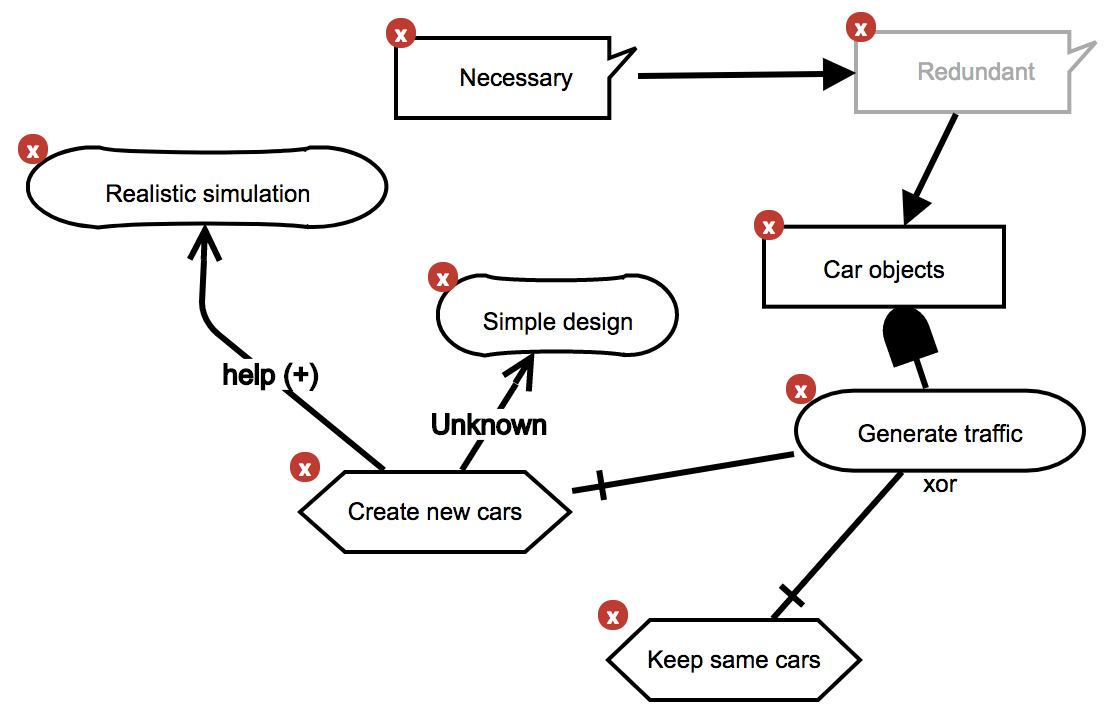
\includegraphics[scale=0.6]{img/tool-figfrompaper}
\caption{RationalGRL model of Figure~\ref{fig:example-small2} in the tool}
\label{fig:tool:figfrompaper}
\end{figure}

\begin{figure}[ht]
\centering
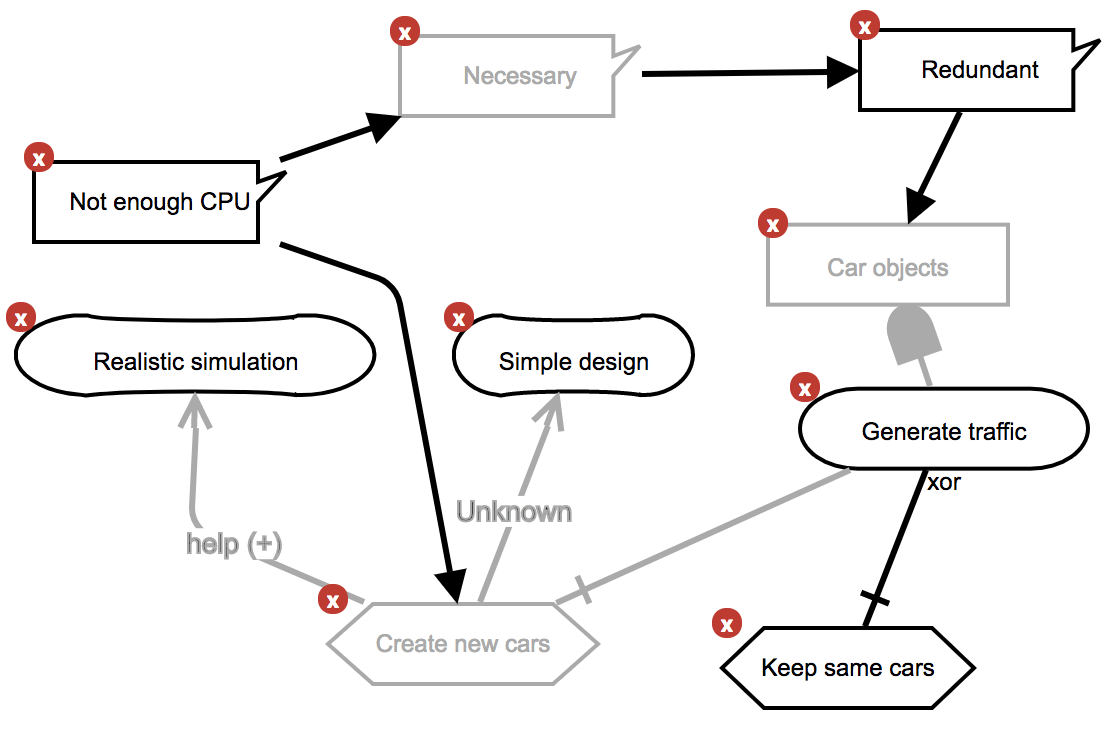
\includegraphics[scale=0.6]{img/tool-multipleattack}
\caption{Adding argument attack multiple arguments to Figure~\ref{fig:tool:figfrompaper}}
\label{fig:tool:multipleattack}
\end{figure}

\end{document}